\chapter{Linear Algebra and Neural Networks}\label{ch_linear_algebra}
\chapterauthor{Jeff Yoshimi, Scott Hotton}

% Also see "indexing hell" comment at  http://neuralnetworksanddeeplearning.com/chap2.html

% Identity matrix

% NN discovers faster matrix product: https://www.nature.com/articles/s41586-022-05172-4. Oddly meta.

In this chapter, we review some basic concepts of linear algebra with an 
emphasis on how they can be applied to the study of neural networks. This can be viewed as a transition from the formal structure of single nodes and weights, to the formal structure of \emph{lists} and \emph{tables} of nodes and weights. In particular, we  consider vectors and matrices, which allow us to describe the behavior of groups of nodes and weights in a compact way.

Linear algebra also facilitates a powerful geometric framework for \emph{visualizing} the structure and dynamics of a neural network. The properties of a set of inputs and whether they can be properly classified is an example of something that is  more intuitively understandable when the input vectors are visualized as points in a space. Chapter \extref{ch_act_functions} notes that whenever the ``play''  button 
\includegraphics[scale=.5]{./images/Play.png} is pressed in Simbrain, some dynamical process is simulated. The framework of linear algebra makes it possible to visualize the changing activations of a set of nodes, or the changing strengths of a set of weights, as a moving point in a space. This approach to thinking about neural networks uses \emph{dynamical systems theory}, discussed in chapter \extref{ch_dst}, and can be used to think about many features of neural network models in an intuitive way.\footnote{For a quick demonstration of this way of visualizing network dynamics, try running the simulation \emph{highDimensionalProjection.bsh}. The dynamics of the network is visible in the projection component.}  

\section{Vectors and Vector Spaces}\label{sect_vector}

% This needs to be done in an intuitive way first, then formalized
    Linear algebra is the study of vector spaces. Vector spaces are abstract
mathematical systems that turn out to be extremely useful for describing the 
structure and dynamics of neural networks. A \glossary{vector space} is a 
collection of objects called \glossary{vectors} along with mathematical 
operations that we can perform with the vectors.\footnote{You may have heard 
that vectors are geometric objects that have a magnitude and a direction. You 
may have seen them represented by an arrow or directed line segment. These 
different points of view on vectors supplement rather than contradict each 
other.}  For instance, we can add two vectors together to get another vector. There is also a type of 
multiplication that can be performed between a vector and a \glossary{scalar}. The term ``scalar'' is used for those numbers that are allowed to be 
multiplied with a vector. We will focus on the case where scalars are real numbers, like $2$, $-1.2$, or $5.9$. If the scalars are the set of real numbers, then the 
vector space is called a {\em real vector space}. We will only work with real
vector spaces. A more formal definition for a vector space is discussed in 
Sect. \ref{S:LinearAlgebraAppendix}. 

We will represent vectors as ordered lists of scalars.\footnote{ Many classes of mathematical objects satisfy the formal definition
of a vector space, and thus many objects can be vectors. The ordered lists we consider here are an especially convenient type of vector.} Each of the scalars in the list is called a \glossary{component} 
of the vector. A list with 2 components is called an {\em ordered pair}. A 
list with 3 components is called an {\em ordered triple}. More generally, a
list with $n$ components is called an {\em $n$-tuple}. We can refer to the
members of a vector in this sense  as its ``first component'',  ``second component'', etc.
A vector in the sense of an $n$-tuple is often 
written out as a comma-separated list of numbers surrounded by parenthesis. 
For example, here are four vectors:
\begin{equation*}
    (0,0) \quad (0,1) \quad (1,0) \quad (1,1) 
\end{equation*}

% TODO: Expand this as we use this more and decide if any convention regarding indices should be given now.
   We sometimes adopt the convention of writing vectors using bold-faced 
lower-case letters, for example $\mathbf{a}_i$ for a  vector of input values, 
$\mathbf{t}$ for a vector of target values, or $\mathbf{a}_4$ for the 
activation vector in the fourth node-layer of a feed-forward network.  By 
contrast non bold-faced, italic lower-case letters are usually reserved for 
components of vectors, and the subscript indicates which component. For 
example, $a_2$ could designate the second component of an activation vector 
$\mathbf{a}$.

When the components of a vector are written horizontally, from left to right,
it is called a {\em row vector}. The ordered pairs shown above are row 
vectors. The components can also be written out vertically, from top to 
bottom, in which case the vector is called a {\em column vector}.\footnote{The choice of whether
to use a row or a column vector to represent an abstract vector is primarily a matter of 
convenience or convention.} Commas are usually 
not written in column vectors because it is clear what the components are. For 
example, here are four column vectors:
\begin{small}
\begin{equation*}
\begin{pmatrix}
0 \\
0
\end{pmatrix} 
\quad 
\begin{pmatrix}
0 \\
1
\end{pmatrix} 
\quad 
\begin{pmatrix}
1 \\
0
\end{pmatrix} 
\quad 
\begin{pmatrix}
1 \\
1
\end{pmatrix} 
\end{equation*}
\end{small}
The number of components in a vector can be any positive integer. If there is
only one component, then the vector is essentially just a scalar.

   For any positive integer $n$, the set of all $n$-tuples forms a vector space.
The integer $n$ is called the \glossary{dimension of a vector space}. For 
example, the set of all of ordered pairs of real numbers is a 2 dimensional 
real vector space $\real^2$. The set of all ordered triples is a 3 dimensional real 
vector space $\real^3$. The set of all possible activations for a network with 172 nodes is a subset of  $\real^{172}$.

   The components of a vector can be thought of as the coordinates of a point
in Euclidean geometry. The components of a vector can be used to locate a
point by starting at the origin and moving parallel to each axis by the 
amount specified by the corresponding component. To locate the point corresponding to the vector 
$(3,4)$, for example, we move $3$ units to the right along the 
horizontal axis and $4$ units upwards along the vertical axis. In this way a 
2 dimensional real vector space can be thought of as an Euclidean plane (see 
figure \ref{2d}).\footnote{There is a legend (probably fabricated, but pedagogically useful nonetheless) 
that the philosopher Ren{\'{e}} Descartes 
 came up with his proof that given a point in the plane there are unique coordinates for that 
 point (and given a pair of coordinates there is a unique point in the plane) 
 while observing flies on his ceiling. He 
 noticed that the position of the flies on the ceiling could be described by 
 superimposing a kind of grid on the ceiling---for example: there's a fly at 
 $(3,4)$, 3 units to the right, and 4 units up; there's a fly at 
 $(-2,-1)$, 2 units to the left, and 1 unit down; and there's another at 
 $(4,-2)$, 4 units to the right, and two units down (see figure \ref{2d}).} 
 
 % This is useful in Simbrain but the connection is a bit lost here 
For 2-dimensional spaces, finding your way around is a bit like using an ``Etch a sketch'' toy\footnote{\url{https://en.wikipedia.org/wiki/Etch_A_Sketch}.}, where you move a tracing point around in a space using one knob for left-and-right ($x$-values) and one knob for up and down ($y$-values). If you plot the activation space of two nodes in Simbrain and adjust the activations of the two nodes, this analogy is useful for understanding what is happening.

\begin{figure}[h]
\centering
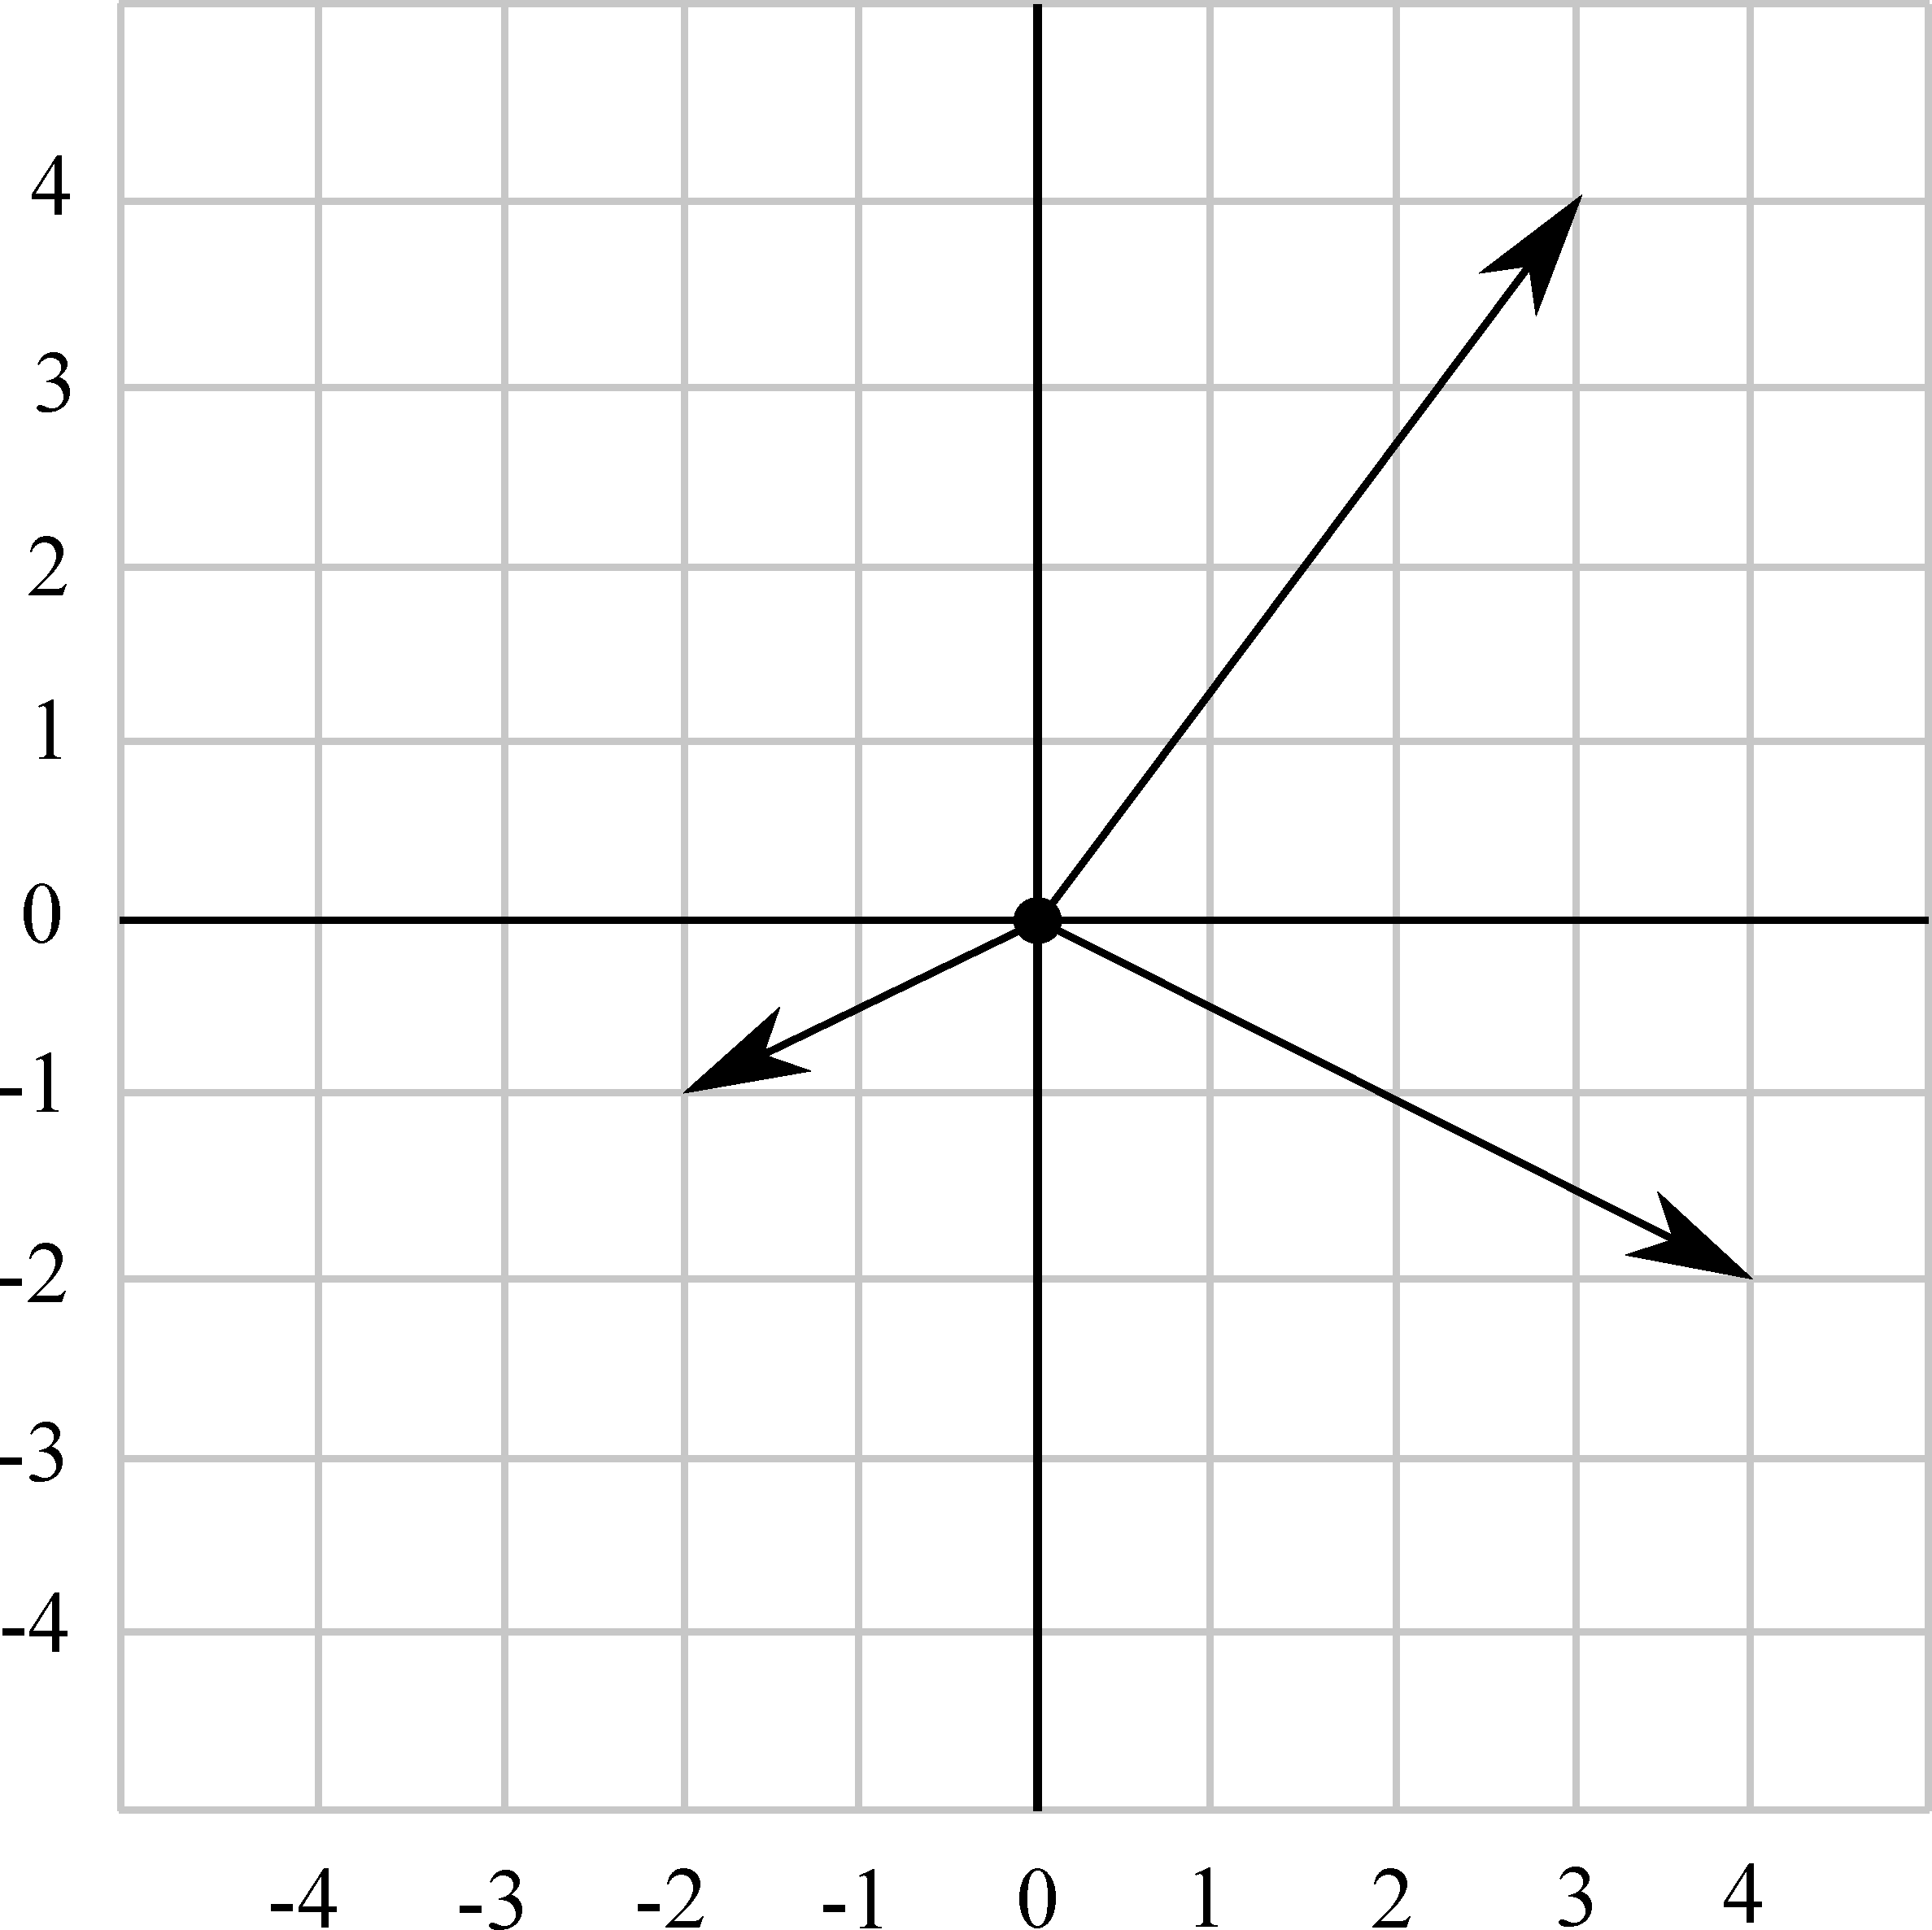
\includegraphics[scale=0.175]{./images/grid2.png}
\caption[Scott Hotton.]{Each vector in a 2 dimensional vector space is associated to a point 
in the Euclidean plane by treating the components of the vector as the 
coordinates of the point. Try to find the vectors $(3,4)$, $(-2,-1)$, and 
$(4,-2)$.} 
\label{2d}
\end{figure}

   The number of dimensions of the vector spaces that arise in the study of 
neural networks can be much larger than 3. We we can not geometrically visualize these higher-dimensional spaces directly. To work mathematically in 
these spaces, it is helpful to keep in mind that our starting point is the 
$n$-tuples, which are just lists of numbers. From this standpoint, the 4 
dimensional real vector space we work with is just the set of all $4$-tuples of
real numbers, and the 5 dimensional real vector space we work with is just the 
set of all $5$-tuples of real numbers. Here are some vectors in a 5 
dimensional vector space:
\begin{equation*}
    (0,-1, 1, 0.4, 9)  \qquad
    (-1, 2, 4, -3, 9)  \qquad 
    (0, 0, 0, -1, -1 ) \qquad
    (0, -1, 0, -1, 0 ) 
\end{equation*}
We can keep going. The vectors that make up a 100 dimensional vector space are 
just lists of 100 numbers. The vectors that make up a billion dimensional 
vector space are just lists of a billion numbers. 

   Real vector spaces with more than 3 dimensions cannot be seen directly, but 
objects in them can be \emph{projected} to lower dimensional real vector spaces 
where they can be visualized. We will discuss methods of projection from 
spaces with more than 3 dimensions in Sect. \ref{S:dimReduction}.\footnote{Here
again the Simbrain simulation \emph{highDimensionalProjection.bsh} is helpful.
When you run the simulation, a sequence of points in a 25 dimensional space 
appears. Each point corresponds to a vector. If you hover the cursor over any
one of the points, you will see the list of 25 numbers (the 25 activation levels
for the network) that correspond to that point.}

\section{Vectors and Vector Spaces in Neural Networks}\label{S:dimReduction}

   Vectors are frequently used to describe lists of activations, weights, and other quantities associated with neural networks. 

\begin{figure}[h]
\centering
\raisebox{-0.5\height}{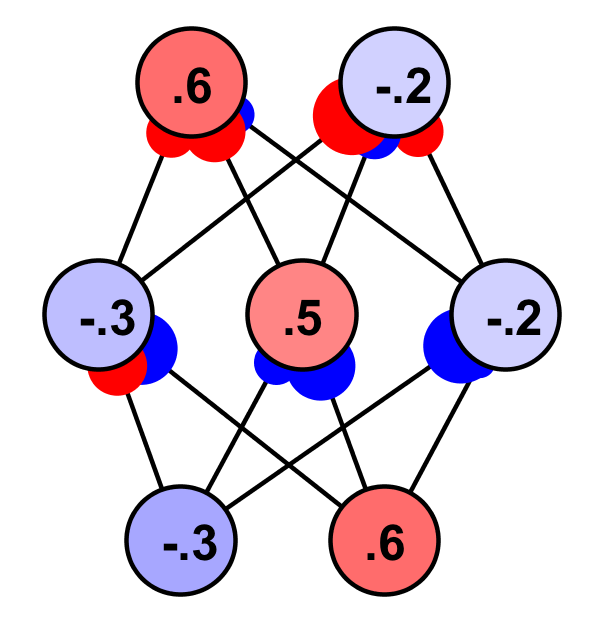
\includegraphics[scale=.5]{./images/ff.png}}
\hspace*{1in}
\raisebox{-0.5\height}{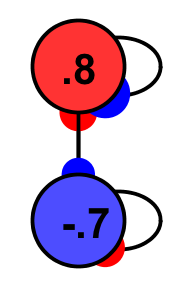
\includegraphics[scale=.3]{./images/recurrent.png}}
\caption[Simbrain screenshots.]{A feed forward and recurrent network in Simbrain. Try to identify the dimensionality of the activation space, input space, hidden unit space, output space, and weight spaces of each network. Left: A feed-forward neural network with activations showing. Right: A 2-node recurrent network with activations showing.}
\label{ffRecurrent}
\end{figure}

% TODO: Run the bold-faced notation through
  The activations of a neural network's $n$ nodes can be described by an \glossary{activation 
vector} with $n$ components, one for each activation value. For example, if we index the nodes of the feed-forward network in figure \ref{ffRecurrent} (Left) from the bottom to the top and left to right (as in figure \ref{labelledNets}), then that networks' activation vector is $(-0.3,0.6,-0.3,0.5,-0.2,0.6,0.2)$. This 
is a vector in a 7 dimensional vector space. A vector space of activation 
vectors is called an \glossary{activation space}. The feed-forward network in figure \ref{ffRecurrent} (Left)  network has a 7 dimensional activation space.

Activation spaces are especially useful in studying recurrent networks. If we index the nodes of the recurrent network in figure \ref{ffRecurrent} (Right) from top to bottom (as in figure \ref{labelledNets}), then its activation vector is $(0.8,-0.7)$. This is a vector in a 2 dimensional activation
space. As the network changes, its activations change, and so we have a changing activation vector. We can picture  this as a moving point in a 2 dimensional space. 

% Promote hidden unit space to glossary / bold
In addition to describing the state of all of a network's nodes by an activation vector, we can describe certain {\em subsets} of its nodes using activation vectors. In the feed-forward network in figure \ref{ffRecurrent} (Left), for example, we can describe the activations of the input nodes as an  \emph{input vector}  $(-0.3,0.6)$  in a 2 dimensional \glossary{input space}. We can describe the activations of the hidden nodes as a vector $(-0.3,0.5,-0.2)$ in a 3 dimensional 
\emph{hidden unit space}. We can describe activations of the output nodes as an \emph{output vector} $(-0.6,-0.2)$ in a 2 dimensional \glossary{output space}. Recall from chapter \extref{ch_intro} that a table of data is a simple environment for a neural network. This table will sometimes contain a set of input vectors, which can be thought of as a set of points in the input space of a network. It can also contain a set of target vectors, which describes how we want the network to respond to input vectors by producing specific output vectors. Many problems in neural network theory can be understood in terms of properties of the input and output space.
 
 Vectors and matrices are sometimes referred to in bold-faced letters, with a subscript indicating more information. So an input vector can be $\textbf{a}_{1}$ for node layer 1 or just $\textbf{a}_{input}$

We can also talk about vectors of weights, or \glossary{weight vectors}, which exist in \glossary{weight spaces}. The feed-forward network in figure \ref{ffRecurrent} has 12 weights. The strengths of those weights is given by the vector 
\begin{equation*}
(-2, 1, -1, 0.9, -1, -1.2, 1, -2, 0.7, -1, 2, 2.1)
\end{equation*}
in a 12 dimensional weight space (see figure \ref{labelledNets}). The recurrent network has 4 weights whose current strengths is given by the vector $(1.1,\; 2,\; 1,-2)$ in a 4 dimensional weight space. In the chapters on supervised and unsupervised learning (chapters \extref{ch_supervised} and \extref{ch_unsupervised}), we will see that it can be helpful to think of learning in terms of movement in a weight space. As the weights of a network are changed or ``trained'' we have a moving point in weight space. Points in weight space can be associated with an error value, which makes it possible to define an \emph{error surface} over a weight space. Supervised learning can often be understood as finding low points on this error surface.
% Low priority discussion item: do we need an indexing system for weights such that we can consistently define weight vectors, including fan-in and fan-out weight vectors?   

It can also be useful to talk about a \glossary{fan-in weight vector} (the list of weight strengths for the set of weights attaching to a node), and a \glossary{fan-out weight vector} (the list of weight strengths for the set of weights exiting a node). A version of the networks in figure \ref{ffRecurrent} with zeroed out activations, labeled node indices, and weight strengths  is shown in figure \ref{labelledNets} below. Some sample weight vectors for these networks are:
\begin{eqnarray*}
\mbox{Feed forward network, neuron 3 fan-in} \;  \;  \;  (1,-2) \\
\mbox{Feed forward network, neuron 3 fan-out} \; \; \; (-2,0.9) \\
\mbox{Feed forward network, neuron 7 fan-in} \; \; \;  (0.9,-1,-1.2) \\
\mbox{Recurrent network, neuron 2 fan-in} \; \; \; (1,-2) \\
\end{eqnarray*}

Some of these weight vectors have 2 components, some have 3 components. Of course for larger networks, fan-in and fan-out vectors can be in higher dimensional weight spaces.\footnote{Notice that the fan-in weight vectors for the hidden units of the feed-forward network have the same number of dimensions as the input vectors. The input vectors and hidden layer fan-in weight vectors live in the same vector space. This fact is useful sometimes.}

\section{Dimensionality Reduction}
\label{S:dimred}

% Mention \url{http://hisee.sourceforge.net/about.html}.

   How can we visualize sets of vectors that have more than three components?  For
example here are nine vectors in a 6 dimensional space:
\begin{eqnarray*}
\begin{array}{rrr}
  ( 2,\;~0,\; 0,\; 0,\; 0,\; 0), \quad 
& ( 0,\; 0,\; 2,\;~0,\; 0,\; 0), \quad 
& ( 0,\; 0,\; 0,\; 0,\; 2,\;~0)  \\
  ( 1,\;~1,\; 0,\; 0,\; 0,\; 0), \quad 
& ( 0,\; 0,\; 1,\;~1,\; 0,\; 0), \quad 
& ( 0,\; 0,\; 0,\; 0,\; 1,\;~1)  \\
  ( 1,  -1,\; 0,\; 0,\; 0,\; 0), \quad 
& ( 0,\; 0,\; 1,  -1,\; 0,\; 0), \quad 
& ( 0,\; 0,\; 0,\; 0,\; 1,  -1)
\end{array}
\end{eqnarray*}
We can't directly visualize these vectors since we only live in a 3 dimensional 
world but we can project them down to a lower dimension. Figure
\ref{F:projection} shows the projection of these vectors down to 2 dimensions.
Each vector above corresponds to one point in the figure. Notice that by 
visualizing the points we can immediately see a structure that is very hard if 
not impossible to see just by looking at the list of vectors. This is how we deal with unwieldy high dimensional data. 

% Todo: Smooth writing and update glossary
A projection is a mapping from a higher dimensional space (sometimes called the ``upstairs'' space or ``total space'') to a lower dimensional space (sometimes called the ``downstairs'' or ``base'' space).\footnote{This is not a formal definition but it will suffice for our purposes. Also note that we focus on vector spaces, but the concept of a projection (and of a dimensionality reduction technique) applies to other types of spaces besides vector spaces.} A method for producing a projection is a \glossary{dimensionality reduction} technique. We are all 
familiar with projections insofar as we have seen globes, which are 3 
dimensional objects, projected down to paper, which are 2 dimensional objects. 

    There are different ways of projecting globes to pages, each of which introduces distinct types of distortions. Even so, we still generally get a sense of what of the objects' shapes are. The geometric relationship between 
various regions in 3 dimensional space can be seen by just looking at a 2 
dimensional map. For example, in a standard Mercator projection of the Earth 
(figure \ref{Mercator}), Antarctica and Greenland look huge, and things are 
especially distorted at the two poles, farthest away from the equator.
%Metrically the continents are different but you can tell which is which by the shape (book?)

\begin{figure}[h]
\centering
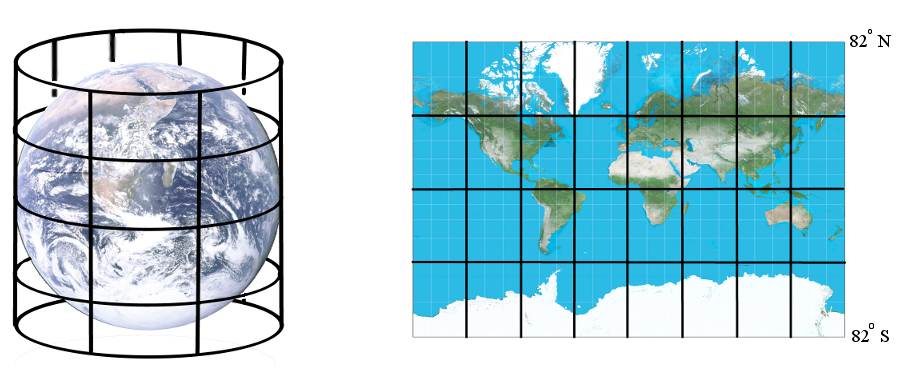
\includegraphics[scale=1.8]{./images/Mercator.jpg}
\caption[Scott Hotton's modification of an image from the Cartographic Research Lab at the University of Alabama.]{The Earth's surface in 3 dimensional space is rendered as a flat, 2
dimensional surface by the Mercator projection method. Most of the distortion
produced by the projection occurs near the Earth's poles so small regions 
around the poles are cropped out from the maps. Most of the continents and
oceans undergo little distortion by the projection which made it a popular 
projection method for making maps of the Earth.} 
\label{Mercator}
\end{figure}
% From https://upload.wikimedia.org/wikipedia/commons/9/97/The_Earth_seen_from_Apollo_17.jpg  AND https://upload.wikimedia.org/wikipedia/commons/f/f4/Mercator_projection_SW.jpg
% Possibly redraw


% The Mercator projection maps the Earth's surace to an infinite strip. It is
% not a radial projection from the center of the Earth, through the Earth, to
% the surrounding cylinder. There are websites that say otherwise but they are wrong.

% For next pass (jeff). Topology is preserved. Distances are not (see Greenland). Abstractly: topology is preserved, but not the metric.

   We can still use the projection to get a sense of the layout of the Earth. 
How are we able to do this?  One reason is that certain {\em topological} 
properties of the Earth's surface--that is, properties involving 
continuity--are preserved by the projection. For example, when we see on the 
map that Los Angeles and San Francisco are on the same coast, then we know we 
can sail along the coast to get from one city to the other. San Francisco is
closer to Merced than it is to Los Angeles, but when we see on the map that 
Merced is not on the coast, then we know that we can not sail from San Francisco 
to Merced. Even though distances on the map have been distorted slightly we 
can still use it to make travel plans. 

% (Jeff notes) Example of spherical pendulum is (almost) a Foucault's penduluum. Like at the observatory. Hanging bob constrained to be on surface of a sphere. Physically familiar. 2 angular coordinates (like lines of latitude and longitude) and 2 velocity coordinates. (Compare regular planar penduluum: circle times line for velocities = tangent bundle for a circle. So 2 dimensional). This 4d thing is tangent  bundle to S2 (which is not S2 x R2). So basically a complex thing that�hard to visualize, since it's not a cartesian product. There is no simple thing to compare it to. // Examples shown is a single surface that contains orbit that maintain the same energy and engular momentum. // Intersection of a level set of the energy function and a level set of the  angular momentum function. //   MAYBE DO IT THIS WAY. Higher dimensional object can't be visualized. We don't know what kind of surface it is. Oh look we can project it to a lower division and see it looks like a torus and is symmetrical. This is a real example that was used in practice. An example of a projection that was actually usefulin practice. A real world example. It did not solve a problem without a solution, but it helped communicate the solution to people who might not otherwise understand the paper. It helps mathematicians understand things that are hard to  understand otherwise. (Ask Scott more about what was revealed.)

   We can use the method of projection to visualize even higher dimensional 
spaces that can not be seen by human eyes. A somewhat exotic example is shown 
on the right of figure \ref{F:projection}. This is the projection of a 2 
dimensional surface in a 4 dimensional space down to a 3 dimensional space. 
The 4 dimensional space is the state space for a spherical pendulum, and the 
surface is the set of all states of the pendulum that have the same energy and 
angular momentum. We can see it resembles the surface of a donut with a groove
along the side. 

   Another example is shown on the left of figure \ref{F:projection}. It 
consists of three circles that intersect at a single point (called a ``bouquet 
of three circles''). In this example, the three circles are perfectly round and 
lie in three mutually perpendicular planes, but we can not see this bouquet of 
circles directly with our eyes. We also can not see, directly with our eyes, 
that this bouquet of circles forms a symmetrical figure in a 6 dimensional 
space. Although the projection distorts the figure a little and we lose some 
of the roundness of the circles in the projected image, we can still see the 
symmetry of the overall figure. The software that was used to do this 
projection is part of Simbrain (the ``projection plot''). This plot can be 
used to visualize structures in the higher dimensional spaces associated with 
many neural networks.

\begin{figure}[h]
\centering
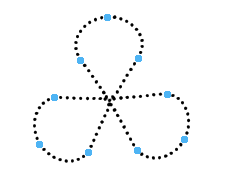
\includegraphics[scale=2.7]{./images/Sammon3.png}
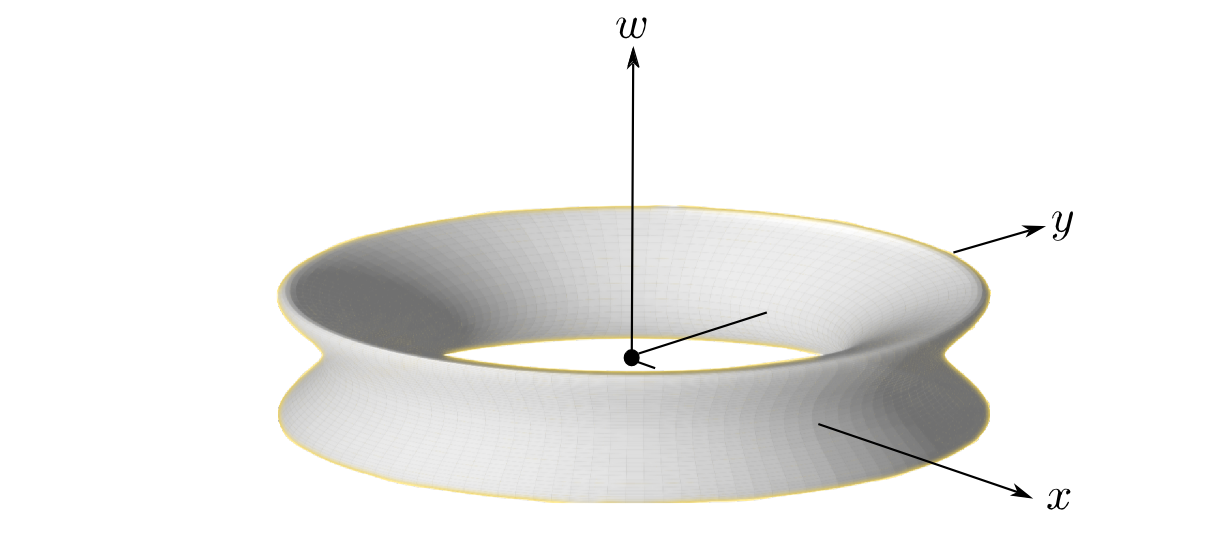
\includegraphics[scale=0.22]{./images/torus.png}
\caption[Scott Hotton.]{(Left) The projection of a symmetrical curve in a 6 dimensional space 
so that we can see its symmetry. The nine vectors listed at the beginning of 
section \ref{S:dimred} are shown as nine large blue dots. (Right) A 
symmetrical surface in a 4 dimensional space is projected so that we can see 
its symmetry.}
\label{F:projection}
\end{figure}

There are many different methods for projecting data from high dimensional spaces to lower dimensional spaces, and the field as a whole is called ``dimensionality reduction''. Each projection method has its pros and cons, and each one introduces different forms of distortion. But by using several such projections one can often get a good sense of the structure of some high dimensional data.\footnote{The three methods used in Simbrain are described here: \url{http://hisee.sourceforge.net/about.html}. Other methods of projection are available in this free Matlab toolbox: \url{http://homepage.tudelft.nl/19j49/Matlab_Toolbox_for_Dimensionality_Reduction.html}.}

\section{The Dot Product}\label{dotProduct}

% Include discussion of orthogonality and closeness from NeuralNets.txt
% If we are doing "distance" on a unit hypersphere, then the dot product  is really an inverse metric. max is 1 then as you go to -1 it is increasingly far away (See that falstad applet to show this).
% The negative cases are important when thinking of a weight vector as orthogonal to a decision boundary  in a network with threshold units
% Why not a definition here if we are going to do it for cosine similarity?

   The \glossary{dot product} is a simple but important function defined for 
pairs of vectors in a vector space.\footnote{The dot product is a member 
of a more general class of functions known as ``inner products''.  They are 
used to specify geometric relationships between vectors.}  The dot product is a 
different kind of function than scalar multiplication (the dot product and 
scalar multiplication are defined in section \ref{S:LinearAlgebraAppendix}).  
They both take two arguments but the types of arguments they take are a little 
different.  The dot product is a function of two vectors that have the same 
number of components, whereas scalar multiplication is a function of a scalar 
and a vector.  The dot product gets its name from the fact it is represented by 
a large dot: $\bullet$.  It is also common to say that we are ``dotting'' one 
vector with another.\footnote{A useful interactive visualization of the dot 
product is available at \url{http://www.falstad.com/dotproduct/}.}
\begin{figure}[h]
\centering
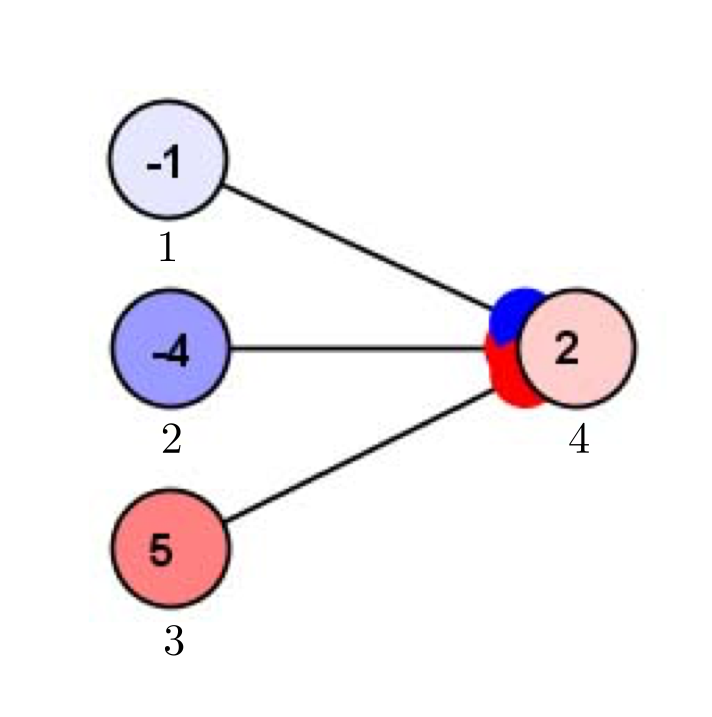
\includegraphics[scale=.7]{./images/Simple3Labelled.png}
\caption[Simbrain screenshot.]{Simple feed-forward network with nodes labeled. 
The dot product can be used to compute the weighted inputs to node 4.} 
\label{F:simplelabelled}
\end{figure}

   The dot product is computed by multiplying each of the corresponding 
components of a pair of vectors, and summing the resulting products.  For 
example
\begin{eqnarray*}
&(1,2,3)  \bullet  (4,5,6)& = \quad 1 \cdot 4 \,+\, 2 \cdot 5 \,+\, 3 \cdot 6 
= 32 \\
&(0,0,0)  \bullet  (4,5,6)& = \quad 0 \cdot 4 \,+\, 0 \cdot 5 \,+\, 0 \cdot 6 
= 0  \\
&(2,3,-1) \bullet (-1,1,1)& = \quad 2 \cdot (-1) \,+\, 3 \cdot 1 \,+\, (-1) 
\cdot 1 = 0 \\
&(1,1,1,1,1) \bullet (1,1,1,1,1)& = \quad  
 1 \cdot 1 \,+\, 1 \cdot 1 \,+\,  1 \cdot 1 \,+\, 1 \cdot 1 \,+\, 1 \cdot 1 = 5
\end{eqnarray*}

   Clearly the product of any vector with the zero vector (the vector whose
components are all $0$) is $0$.  However, the dot product of two non-zero 
vectors can also be $0$.  When the dot product of two non-zero vectors is $0$ 
then we say the vectors are \glossary{orthogonal} (perpendicular) to each 
other.  It might be hard to tell right away that the vectors $(2,-1,1,-3,1,1)$,
and $(1,2,3,1,1,-1)$ are orthogonal to each other, but a quick calculation 
shows us that it is true:
\begin{eqnarray*}
           (2,-1,1,-3,1,1) \bullet (1,2,3,1,1,-1) = 0
\end{eqnarray*}
% The dot product can also be used to uncover other geometric properties in 
% high dimensional spaces.

   Notice that we can concisely represent the weighted input (see chapter 
\extref{ch_act_functions}) to a node using the dot product.  The weighted input 
is just the dot product of the activation vector with the fan-in weight vector 
of the output node, plus a bias term.  An example is shown in figure 
\ref{F:simplelabelled}.  The activation vector for nodes $1$, $2$, and $3$ is 
$(\; -1,\; -4,\; 5)$ and the weight vector for node $4$ is $(-1,-1,1)$ so the 
net-input to node $4$ is:
\begin{equation*}
n_4 = (\; -1,\; -4,\; 5) \bullet (-1,-1,1) + 0  = 1 + 4 + 5 + 0 = 10
\end{equation*}

   These visualizations help show that if we are doing ``distance'' on a unit hypersphere, then the dot product behaves like an inverse metric: it reaches a maximum of 1 when vectors point in the same direction, and becomes increasingly negative as they point in opposite directions. The negative cases are especially important when thinking of a weight vector as orthogonal to a decision boundary in a network with threshold units.
 
\section{Other vector comparison methods}\label{vector_comparisons}

   There are a number of ways the dot product can be used to give us a sense of
how close or far apart two vectors (such as input vectors, activation vectors, 
\emph{etc}.) are to each other.  

% Can't this be expressed as cos(u,v)?  
% It can be, but its not common.

   One way is to begin by normalzing the two vectors (that is, we divide each
of the vectors by their Euclidrean norm to get two vectors with unit norm; see 
section \ref{metricSpace}).  We then dot the normalized vectors with each 
other.\footnote{The symbol $||\cdot||$ denotes the Euclidean norm.}
\begin{equation}\label{E:cossim}
\cos(\theta) = 
\frac{\mathbf{u}}{|| \mathbf{u}||}  \bullet 
\frac{\mathbf{v}}{|| \mathbf{v}||} =
\frac{\mathbf{u} \bullet \mathbf{v}}{|| \mathbf{u}||  \cdot 
||\mathbf{v}||}
\end{equation}
This normalized dot product is known as \glossary{cosine similarity}.  It is a 
commonly used measure of similarity that is independent of the vector's 
magnitude.  The number $\theta$ is the angle between $\mathbf{u}$ and 
$\mathbf{v}$.  The cosine of the angle between the vectors tells us the extent 
to which the vectors point in the same direction.  The cosine similarity of two 
vectors can be any number in the interval $[-1, 1]$.  If the vectors point in 
exactly the same direction then the angle between them is $0$ and their cosine 
similarity $1$.  If the vectors are orthogonal to each other then the angle 
between them is $90^o$ and their cosine similarity is $0$.  If the vectors 
point in directly opposite directions then the angle between them is $180^o$ 
and their cosine similarity is $-1$.\footnote{In some implementations the
quantity is bounded between $[0,1]$.  Occasionally, cosine distance is used, 
which is $1 - \cos(\theta)$.  In this case nearly proportional vectors 
will have a cosine distance of nearly 0, while very dissimilar vectors will 
have a cosine distance of about 1.}

   Note that we do not need to know the angle $\theta$ to compute the
cosine similarity of two vectors.\footnote{In fact in modern Euclidean geometry 
angles are formally defined in terms of the dot product.}  Cosine
similarity can be computed for any pair of vectors in the same vector space no 
matter how many dimensions the vector space has, although it does take more
time to compute it in higher dimensions.  Even though the left hand side of 
equation \eqref{E:cossim} is only a function of the angle between the vectors 
the cosine similarity of any two nonzero vectors, $\mathbf{u}$ and 
$\mathbf{v}$, can be computed from the expression on the right hand side of 
equation \eqref{E:cossim}.

   Cosine similarity is widely used in text analysis and natural language 
processing, especially in applications such as document similarity and 
information retrieval (see chapter \extref{ch_word_embeddings}).  This is 
because it compares the direction of two high-dimensional vectors independently
of their magnitude.  As such, it captures similarity in content rather than 
length or scale, which is ideal in contexts where longer documents might 
contain similar themes as shorter ones.
% Last point should be front-loaded a bit?

   Two other related measures are \textbf{covariance} and \textbf{correlation}.
In this context it can be helpful for us to consider the two vectors as 
sequences of values for two variables.  Covariance and correlaation measure how 
closely the two variables vary together about each of their respective means.  
If, at each moment in time, the variables are usually either both above or both 
below their mean values then we say the variables are positively correlated 
with each other.  When the variables are positively correlated and we see that
the value for one of them is above average then the value for the other 
variable is probably also above average.  On the other hand if both variables 
are usually on opposite sides of their mean values then we say the variables 
are negaatively correlated with each other.  When the variables are negatively 
correlated and we see that the value for one of them is above average then the 
value for the other variable is probably below average.  If the variables are
neither positively or negatively correlated then we say they are uncorrelated.

Covariance measures how closely two variables vary together about each of their
means.  Correlation does the same thing but it also rescales the result to 
produce a standardized value between in $[-1,1]$.  To compute the covariance 
between two raw data vectors $\mathbf{x} = (x_1, \dots, x_n)$ and $\mathbf{y} =
(y_1, \dots, y_n)$, we first subtract the mean value of each vector from 
its components to obtain centered data vectors:
\begin{eqnarray}
\tilde{\mathbf{x}} &=& (x_1 - \bar{x}, \, \dots, \, x_n - \bar{x}) 
                                                             \nonumber \\[1mm]
\tilde{\mathbf{y}} &=& (y_1 - \bar{y}, \, \dots, \, y_n - \bar{y}) 
\end{eqnarray}
The covariance is the dot product of the centered data vectors divided by
$n-1$.

   Covariance and correlation have exact mathematical expressions.  Let $x$ and 
$y$ stand for the two variables.  A value for each of the variables can be 
obtained at each moment in time by making a measurement or by sampling from a 
large population.  However we obtain values for $x$ and $y$ we get two 
sequences of values for these two variables.  This is called the 
\emph{raw data} for the variables.  The two sequences of values for the 
variables can be expressed as vectors:

\begin{equation}
\mathbf{x} = (x_1, \dots, x_n) \quad \mbox{and} \quad 
\mathbf{y} = (y_1, \dots, y_n)
\end{equation}
To compute the covariance of $\mathbf{x}$ and $\mathbf{y}$ we first subtract 
the mean value of each vector from its components.  We let $\mu_x$ be the 
mean of $\mathbf{x}$ and $\mu_y$ be the mean of $\mathbf{y}$.  This gives 
us two vectors whose components are called the \emph{centered data} for the 
variables.
\begin{eqnarray}
\tilde{\mathbf{x}} &=& (x_1 - \mu_x, \, \dots, \, x_n - \mu_x) 
                                                             \nonumber \\[1mm]
\tilde{\mathbf{y}} &=& (y_1 - \mu_y, \, \dots, \, y_n - \mu_y) 
\end{eqnarray}
The covariance is the dot product of the vectors for the centered data divided 
by $n$.\footnote{Sometimes $n-1$ is used instead of $n$.}
\begin{equation}\label{E:covdef}
\mathrm{Cov}(\mathbf{x}, \mathbf{y}) = \frac{\tilde{\mathbf{x}} \bullet 
                                             \tilde{\mathbf{y}}}{n} 
\end{equation}

   The Pearson correlation coefficient is obtained from the covariance using
the standard deviations of the variables.  The standard deviation, like the 
mean, is a statistic intended to describe the raw data.  It describes how 
spread out the raw data is.  The standard deviation for $x$ and $y$ are defined
as:
\begin{equation}
    \sigma_x = \sqrt{ \frac{1}{n} \sum_{j=1}^n (x_j - \mu_x)^2} 
\qquad \mbox{and} \qquad 
    \sigma_y = \sqrt{ \frac{1}{n} \sum_{j=1}^n (y_j - \mu_y)^2}
\end{equation}
The Pearson correlation coefficient is the covariance divided by the product of
the standard deviations.
\begin{equation}\label{E:corrdef}
\mathrm{Corr}(\mathbf{x}, \mathbf{y}) = 
\frac{\mathrm{Cov}(\mathbf{x}, \mathbf{y})}{\sigma_x \, \sigma_y}
\end{equation}
However we can also write the standard deviation in terms of the centered data:
\begin{equation}\label{E:stddevc}
  \sigma_x = \sqrt{ \frac{\tilde{\mathbf{x}} \bullet \tilde{\mathbf{x}}}{n}}
= \frac{||\tilde{\mathbf{x}}||}{\sqrt{n}}
\qquad \mbox{and} \qquad 
  \sigma_y = \sqrt{ \frac{\tilde{\mathbf{y}} \bullet \tilde{\mathbf{y}}}{n}}
= \frac{||\tilde{\mathbf{y}}||}{\sqrt{n}}
\end{equation}
We can substitute the formula for the covariance in equation \eqref{E:covdef},
and the formulas for the standard deviations in equation \eqref{E:stddevc}
into the right had side of equation \eqref{E:corrdef}.
\begin{equation}
\mathrm{Corr}(\mathbf{x}, \mathbf{y}) = 
\frac{\left(\displaystyle{\frac{\tilde{\mathbf{x}} \bullet 
                                                 \tilde{\mathbf{y}}}{n}}\right)}
     {\left(\displaystyle{\frac{||\tilde{\mathbf{x}}||}{\sqrt{n}}
               \frac{||\tilde{\mathbf{y}}||}{\sqrt{n}} }\right)}
= \frac{\tilde{\mathbf{x}} \bullet \tilde{\mathbf{y}}}
       {||\tilde{\mathbf{x}}|| \cdot ||\tilde{\mathbf{y}}||} 
\end{equation}
So we can see that the Pearson correlation coefficient of the raw data is the
same as the cosine similarity of the centered data.  It is a number in 
$[-1,1]$.  

   Covariance and correlation have exact mathematical expressions.  Let $x$ and 
$y$ stand for the two variables.  A value for each of the variables can be 
obtained at each moment in time by making a measurement or by sampling from a 
large population.  However we obtain values for $x$ and $y$ we get two 
sequences of values for these two variables.  This is called the 
\emph{raw data} for the variables.  The two sequences of values for the 
variables can be expressed as vectors:
\begin{equation}
\mathbf{x} = (x_1, \dots, x_n) \quad \mbox{and} \quad 
\mathbf{y} = (y_1, \dots, y_n)
\end{equation}
To compute the covariance of $\mathbf{x}$ and $\mathbf{y}$ we first subtract 
the mean value of each vector from its components.  We let $\mu_x$ be the 
mean of $\mathbf{x}$ and $\mu_y$ be the mean of $\mathbf{y}$.  This gives 
us two vectors whose components are called the \emph{centered data} for the 
variables.
\begin{eqnarray}
\widetilde{\mathbf{x}} &=& (x_1 - \mu_x, \, \dots, \, x_n - \mu_x) 
                                                             \nonumber \\[1mm]
\widetilde{\mathbf{y}} &=& (y_1 - \mu_y, \, \dots, \, y_n - \mu_y) 
\end{eqnarray}
The covariance is the dot product of the vectors for the centered data divided 
by $n$.\footnote{Sometimes $n-1$ is used instead of $n$.}
\begin{equation}\label{E:covdef}
\mathrm{Cov}(\mathbf{x}, \mathbf{y}) = \frac{\widetilde{\mathbf{x}} \bullet 
                                             \widetilde{\mathbf{y}}}{n} 
\end{equation}

   The Pearson correlation coefficient is obtained from the covariance using
the standard deviations of the variables.  The standard deviation, like the 
mean, is a statistic intended to describe the raw data.  It describes how 
spread out the raw data is.  The standard deviation for $x$ and $y$ are defined
as:
\begin{equation}
    \sigma_x = \sqrt{ \frac{1}{n} \sum_{j=1}^n (x_j - \mu_x)^2} 
\qquad \mbox{and} \qquad 
    \sigma_y = \sqrt{ \frac{1}{n} \sum_{j=1}^n (y_j - \mu_y)^2}
\end{equation}
The Pearson correlation coefficient is the covariance divided by the product of
the standard deviations.
\begin{equation}\label{E:corrdef}
\mathrm{Corr}(\mathbf{x}, \mathbf{y}) = 
\frac{\mathrm{Cov}(\mathbf{x}, \mathbf{y})}{\sigma_x \, \sigma_y}
\end{equation}
It is a number in $[-1,1]$.  If $\mathrm{Corr}(\mathbf{x}, \mathbf{y})$ is 
close to $1$ then $\mathbf{x}$ and $\mathbf{y}$ are highly positively 
correlated.  If $\mathrm{Corr}(\mathbf{x}, \mathbf{y})$ is close to $-1$ then 
$\mathbf{x}$ and $\mathbf{y}$ are highly negatively correlated.  If 
$\mathrm{Corr}(\mathbf{x}, \mathbf{y})$ is close to $0$ then $\mathbf{x}$ and 
$\mathbf{y})$ are nearly uncorrelated.  

   We can also write the standard deviation in terms of the centered data:
\begin{equation}\label{E:stddevc}
  \sigma_x = \sqrt{ \frac{\widetilde{\mathbf{x}} \bullet \widetilde{\mathbf{x}}}{n}}
= \frac{||\widetilde{\mathbf{x}}||}{\sqrt{n}}
\qquad \mbox{and} \qquad 
  \sigma_y = \sqrt{ \frac{\widetilde{\mathbf{y}} \bullet \widetilde{\mathbf{y}}}{n}}
= \frac{||\widetilde{\mathbf{y}}||}{\sqrt{n}}
\end{equation}
We can substitute the formula for the covariance in equation \eqref{E:covdef},
and the formulas for the standard deviations in equation \eqref{E:stddevc}
into the right had side of equation \eqref{E:corrdef}.
\begin{equation}
\mathrm{Corr}(\mathbf{x}, \mathbf{y}) = 
\frac{\left(\displaystyle{\frac{\widetilde{\mathbf{x}} \bullet 
                                            \widetilde{\mathbf{y}}}{n}}\right)}
     {\left(\displaystyle{\frac{||\widetilde{\mathbf{x}}||}{\sqrt{n}}
               \frac{||\widetilde{\mathbf{y}}||}{\sqrt{n}} }\right)}
= \frac{\widetilde{\mathbf{x}} \bullet \widetilde{\mathbf{y}}}
       {||\widetilde{\mathbf{x}}|| \cdot ||\widetilde{\mathbf{y}}||} 
\end{equation}
So we can see that the Pearson correlation coefficient of the raw data is the
same as the cosine similarity of the centered data.  The correlation of 
$\mathbf{x}$ and $\mathbf{y}$ corresponds to the extent to which 
$\widetilde{\mathbf{x}}$ and $\widetilde{\mathbf{y}}$ point in the same 
direction.

    Geometrically, the centered data $\widetilde{\mathbf{x}}$ and 
$\widetilde{\mathbf{y}}$, are the orthogonal projections of the raw data 
$\mathbf{x}$ and $\mathbf{y}$ to the subspace orthogonal to the vector 
$(1, \dots, 1)$.  This subsapce has dimension $n - 1$.  This projection 
never increases the angle between $\mathbf{x}$ and $\mathbf{y}$ but it can 
descrease angle between them.  In a sense, there are fewer ways they can point 
away from each other when we reduce the number of dimensions by $1$. 

    Geometrically, the centered data $\tilde{\mathbf{x}}$ and 
$\tilde{\mathbf{y}}$, are the orthogonal projections of the raw data 
$\mathbf{x}$ and $\mathbf{y}$ to the subspace orthogonal to the vector 
$(1, \dots, 1)$.  This subsapce has dimension $n - 1$.  This projection 
never increases the angle between $\mathbf{x}$ and $\mathbf{y}$ but it can 
descrease angle between them.  In a sense, there are fewer ways they can point 
away from each other when we reduce the number of dimensions by $1$. 

   The vectors $\mathbf{x}$ and $\mathbf{y}$ can represent different physical 
quantities whose numerical value depends on the choice of units of measure.
By centering the data before computing the cosine similarity we avoid spurious 
differences introduced by the units of measure.  For example, suppose we are 
measuring the germination time of seeds as a function of temperature.  If we 
measure temperature in Celsius and time in seconds, we will obtain a different 
numerical value for the cosine similarity of the raw data than if we measure 
time in hours.  Whereas the value of the Pearson correlation coefficient 
remains the same regardless of such changes in the unit of measure. 
value for the cosine similarity than if we measure time in hours.  Whereas the 
value of the Pearson correlation coefficient remains the same regardless of 
such changes in the unit of measure. 

   These four measures—dot product, cosine similarity, covariance, and 
correlation—are closely related.  They all associate pairs of vectors with 
scalars.  They can be distinguished by whether they center the vectors (by 
subtracting the mean) and /or scale them (by dividing dividing by the 
``spread'' of the data) before comparison.  The dot product operates on the raw
data directly, while the other three measure transform the raw data in 
different ways to faciltate comparisons between data with different means or 
overall scales.

\begin{itemize}
    \item \textbf{Dot product}: not centered, not scaled.
    \item \textbf{Cosine similarity}: not centered, scaled.
    \item \textbf{Covariance}: centered, not scaled.
    \item \textbf{Correlation}: centered, scaled.
\end{itemize}

   It's worth noting that different comparison measures often arise from 
different  approaches to the data.  The easiest way to see this is by 
considering a table.  Recall from chapter \extref{ch_data_science} that tables 
are commonly used in neural networks and the columns often describe some
features of interest.   

   Let us consider this table of data.
\begin{center}
\begin{tabular}{ccc}
\textbf{Individual} & \textbf{Height (ft)} & \textbf{Weight (lb)} \\
\hline
1 & 5.0 & 120 \\
2 & 5.5 & 180 \\
3 & 6.5 & 210 \\
4 & 6.0 & 150 \\
5 & 5.8 & 170 \\
\end{tabular}
\end{center}
There are two main ways to think geometrically about the numbers in this table.
One way is to let the ordered pairs of heights and weight in the five rows of 
the table be the coordinates of five points in $\real^2$.  Since this space 
only has 2 dimensions we can visualuze these points.  In this point of view 
the heights and weights being positively correlated means that these five 
points are nearly collinear to a line with positive slope in the plane.  When 
the heights and weights are negatively correlated it means that the points are 
nearly collinear to a line with negative slope in the plane.  When the heights 
and weights are uncorrelated they usually form a cloud of points in $\real^2$ 
\label{twogeoms}

   The left panel of figure \ref{twogeoms} shows the five points in $\real^2$.
The Pearson correlation coefficint for them is about $0.8$.  They are roughly 
collinear to a line with positive slope.

\begin{figure}[h]
\centering
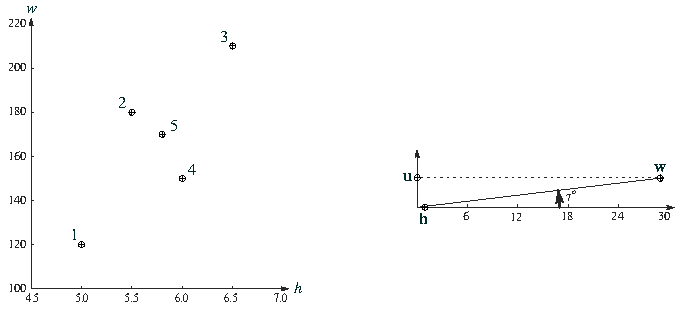
\includegraphics[scale=1.25]{./images/heightWeight.pdf}
\caption{(left) The height and weight coordinates for the five individuals in
the table.  The odd numbered points are nearly collinear to a line with a
slope of about $60$ while the even numbered points are more spread out.
(right)  The vector $\mathbf{h}$ points to the right in the horizontal 
direction while the vector $\mathbf{u}$ points in the upward vertical 
direction.  The length of $\mathbf{u}$ is about $3.5$ times the length of 
$\mathbf{h}$ and the length of $\mathbf{w}$ is about $8$ times the length of
$\mathbf{u}$.  The cosine similarity of $\mathbf{h}$ and $\mathbf{w}$ is about 
0.9925 and the angle between $\mathbf{h}$ and $\mathbf{w}$ is about $7^o$.} 
\label{twogeoms}
\end{figure}

   The other main way to think geometrically about the numbers in the table is 
to let the columns for the heights and weights be the coordinates for two 
points in $\real^5$.  Since this space has 5 dimensions we can not visualize 
these points directly but we do have the advantage in this case that there are 
only two points so they have to be contained within a 2 dimensional subspace
of $\real^5$.  We represent the heights with the vector 
\begin{equation*}
\mathbf{h} = (5.0,\, 5.5,\, 6.5,\, 6.0,\, 5.8)
\end{equation*}
and the weights with the vector 
\begin{equation*}
\mathbf{w} = (120,\, 180,\, 210,\, 150,\, 170)
\end{equation*}
For the purpose of visualzing the geometrical relationship between 
$\mathbf{h}$ and $\mathbf{w}$ we define another vector
\begin{equation*}
\mathbf{u} = (-24.8187,\, 20.6994,\, 21.7356,\, -23,7825,\, 2.0103)
\end{equation*}
It can be checked that to three digits:
\begin{equation*}
\mathbf{h} \bullet \mathbf{u} \approx 0 \quad \mbox{and} \quad
\mathbf{w} \approx 28.964 \, \mathbf{h} + \mathbf{u}
\end{equation*}
so that $\{ \mathbf{h}, \mathbf{u} \}$ is nearly orthogonal basis for the span
of $\{ \mathbf{h}, \mathbf{w} \}$.  The vector $\mathbf{w}$ is about $30$ 
times as long as the vector $\mathbf{h}$.  This is shown in the right panel of
figure \ref{twogeoms}.


.  The cosine 
similarity of the data gives us the cosine of the angle between the two points 
as measured from the origin of $\real^5$.

In neural network contexts, we frequently focus on the \emph{rows} of such a 
dataset and compare them, for example considering pairs of input vectors or 
activation vectors to assess their similarity.  Often the dot product or cosine 
similarity are used to see if they point in the same direction in an input 
space or activation space.  Often we have many rows and thus many points to 
think about, a cloud points in an abstract space.  By contrast, when computing 
covariance or correlation, we typically work with the \emph{columns}, of such a 
dataset, comparing features like weight and height. We then compute the 
correlation or covariation a single time, getting a single value out of the 
pair of vectors.  Or if we have many columns with many features (suppose we 
also had BMI, resting heart rate, and age in the table above), we might compute 
multiple correlations or covariances.  So in a sense dot product and cosine 
similarity are more row oriented, and correlation and covariance are more 
column oriented.

Given a set of vectors, we can compute all their pairwise relationships using the methods above. Correlation matrices and covariances are well known for this purpose. We refer to these generally as \textbf{vector comparison matrices}. These matrices serve as  tools for exploring similarity, alignment, or statistical dependence among sets of vectors.  It is very helpful to be able to interpret these. They also function as processing elements of some networks, most famously the transformer architecture used in large language models, where the self attention matrix compares vector representations of all the tokens in a context window (see chapter \extref{ch_transformers}).  

Here is an example using pairwise dot products (what is sometimes called a ``Gram matrix''). Suppose we have three vectors in \( \mathbb{R}^3 \):

\[
\mathbf{v}_1 = 
\begin{bmatrix}
1 \\
0 \\
1
\end{bmatrix}, \quad
\mathbf{v}_2 = 
\begin{bmatrix}
0 \\
1 \\
1
\end{bmatrix}, \quad
\mathbf{v}_3 = 
\begin{bmatrix}
1 \\
1 \\
0
\end{bmatrix}
\]

We can construct a dot product matrix by computing every pairwise dot product:

\[
\begin{array}{c|ccc}
 & \mathbf{v}_1 & \mathbf{v}_2 & \mathbf{v}_3 \\
\hline
\mathbf{v}_1 & \mathbf{v}_1 \cdot \mathbf{v}_1 = 2 & \mathbf{v}_1 \cdot \mathbf{v}_2 = 1 & \mathbf{v}_1 \cdot \mathbf{v}_3 = 1 \\
\mathbf{v}_2 & \mathbf{v}_2 \cdot \mathbf{v}_1 = 1 & \mathbf{v}_2 \cdot \mathbf{v}_2 = 2 & \mathbf{v}_2 \cdot \mathbf{v}_3 = 1 \\
\mathbf{v}_3 & \mathbf{v}_3 \cdot \mathbf{v}_1 = 1 & \mathbf{v}_3 \cdot \mathbf{v}_2 = 1 & \mathbf{v}_3 \cdot \mathbf{v}_3 = 2 \\
\end{array}
\]

So we get

\[
=
\begin{bmatrix}
2 & 1 & 1 \\
1 & 2 & 1 \\
1 & 1 & 2 \\
\end{bmatrix}
\]

This matrix shows, for instance, that \( \mathbf{v}_1 \cdot \mathbf{v}_2 = 1 \), indicating 
moderate alignment between those two vectors, and that each vector has a dot product of 2 
with itself (its squared length).

In Simbrain there is a tool that is often useful for comparing a set of vectors to itself in all pairwise combinations, using any of the  methods mentions in this section. It is shown in figure \ref{corrPlot}.

\begin{figure}[h]
\centering
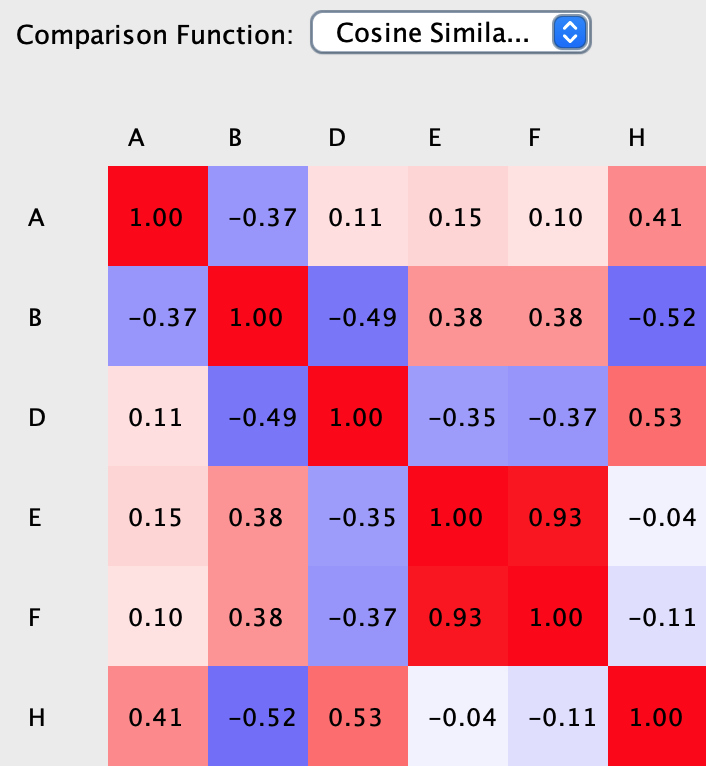
\includegraphics[scale=.5]{./images/corrPlot.png}
\caption[Simbrain screenshot from Jeff Yoshimi.]{A plot in Simbrain that allows a set of vectors (here labeled ``A'', ``B'', etc. They are vectors that correspond to flattened pixel images of letters) to be compared using various vector comparison methods. Any set of vectors can be used to create this kind of plot. The diagonals generally show maximal values for similarity measures, since vectors are on most measures maximally similar to themselves. }
\label{corrPlot}
\end{figure}

% Add some exercises to the end where they construct these

\section{Vector Spaces as Metric Spaces}\label{metricSpace}

% A picture would be nice here
% Should magnitude be mentioned here? 

A vector space can have a metric, which is a way to define the distance between any two points. The usual metric for a real vector space is the Euclidean metric, which can be expressed in terms of the dot product. The Euclidean metric uses the concept of a \glossary{norm}, denoted by double bars $|| \cdot ||$, which measures the ``length'' of a vector. Specifically, the norm of a vector $\mathbf{x}$ is the square root of the dot product of the vector with itself: $||\mathbf{x}|| = \sqrt{\mathbf{x} \bullet \mathbf{x}}$.  With this
metric the distance between any pair of vectors in $\real^n$ is:
\begin{equation*}
\mathbf{x} = (x_1, x_2, \ldots, x_n) \qquad
\mathbf{y} = (y_1, y_2, \ldots, y_n) \qquad
\end{equation*}
is:
\begin{equation*}
|| \mathbf{x} - \mathbf{y} || =
\sqrt{ (\mathbf{x} - \mathbf{y}) \bullet (\mathbf{x} - \mathbf{y}) }
= \sqrt{ \sum_{j=0}^n (x_j - y_j)^2 }
\end{equation*}
There are many metrics for every vector space but usually we use the Euclidean metric.

% Consider adding a plot showing nearby points here.
The upshot of this is that we can interpret the vector spaces associated with neural networks--activation spaces, input spaces, weight spaces, etc.--as giving us a sense of how far apart relevant vectors are, and thus how similar the things they represent are. Points nearby one another in an input space correspond to similar inputs: similar smells, similar visual inputs, similar words relative to a word embedding (chapter \extref{ch_word_embeddings}), etc. Points nearby one another in a weight space are similar configurations of weights. These interpretations are often emphasized in analyses of neural networks (for example, see chapter \extref{ch_representations}), and in fact the spaces associated with neural networks are sometimes called ``similarity spaces''.  An example which illustrates the importance of this way of thinking is figure \extref{competitiveInputSpace}.

\section{Matrices}\label{sect_matrices}

% Officially stipulate our usage: components of a vectors, entries of a matrix.

   Another object studied in linear algebra is a \glossary{matrix}, which is a 
rectangular array of numbers arranged into rows and columns: basically a table of 
values. Here is an example of a matrix:
\[
\begin{pmatrix}
 1  &   9  & 7 \\
 5  &   3  & 2 \\
0.3 &  -1  & 0 \\
 0  & -0.4 & 0
\end{pmatrix}
\]
It is conventional to describe matrices by stating the number of rows and 
columns they have, in that order. The example above is a $4 \times 3$ 
matrix because it has 4 rows and 3 columns.\footnote{The notation for vectors typically includes a comma-separated list of the vector's components. The notation for matrices typically does contain not commas. A  matrix's components are only aligned into rows and columns without any extra characters to separate them. Otherwise we think of vectors as special cases of matrices. A vector with $n$ components can be represented as either a $1 \times n$ matrix or as an $n \times 1$ matrix. So far we have been representing vectors as $1 \times n$ matrices.} This is also called the \glossary{shape} of a matrix.  Each row of a matrix is called a \glossary{row vector} and each column is called a \glossary{column vector}. The matrix above has four row vectors and 
three column vectors.\footnote{Note that vectors  are matrices and matrices are vectors!  As already noted, vectors are a special kind of a matrix, 
a matrix with one row or one column. Conversely, matrices are technically a 
kind of vector, since they satisfy the formal definition of a vector (they 
exist in vector spaces called ``matrix spaces''). However, it will be easier for us to follow standard practice and treat these as separate kinds of mathematical objects.}  

\begin{figure}[h]
\centering
\raisebox{-0.5\height}{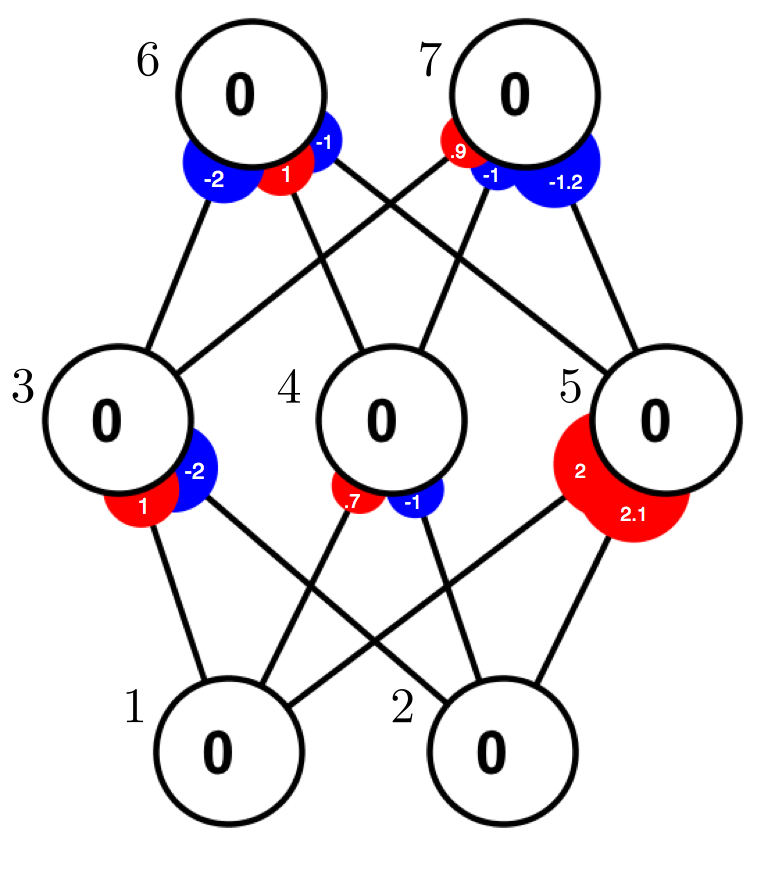
\includegraphics[scale=.45]{./images/ff_labelled.png}}
\hspace*{.7in}
\raisebox{-0.5\height}{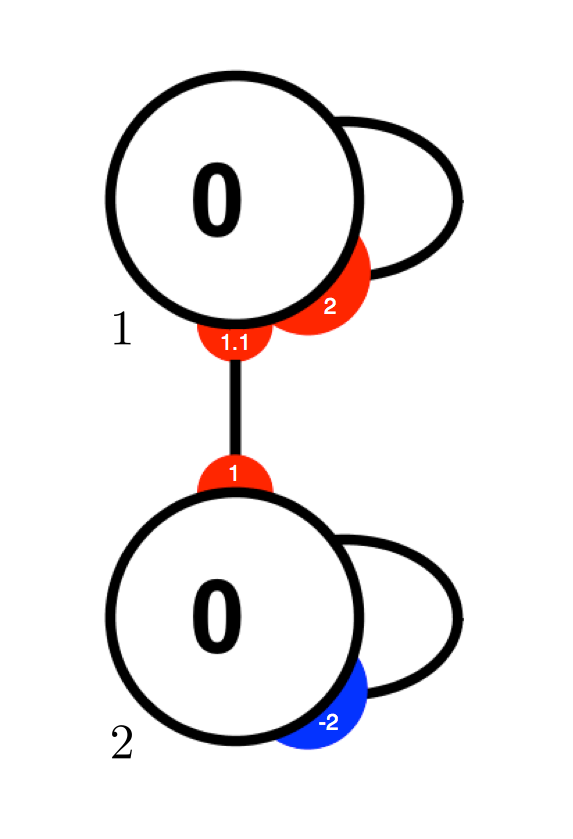
\includegraphics[scale=.2]{./images/recurrent_labelled.png}}
\caption[Simbrain screenshots modified by Jeff Yoshimi.]{Feedforward and recurrent networks with nodes labelled, and weight strengths shown. Each weight layer of the feedforward network and the weights of the recurrent network can be associated with weight matrices. }
\label{labelledNets}
\end{figure}

We adopt the convention of writing matrices using bold-faced upper-case letters, for example $\mathbf{W}$ or $\mathbf{R}$. By contrast, non bold-faced, italic lower-case letters are reserved for entries in a matrix, and subscripts indicate which row and column. For example $w_{2,3}$ could be the scalar at the second row and third column of a $2 \times 3$ matrix $\mathbf{W}$.\footnote{In physics and mathematics it would be more conventional to use upper-case letters like $W_{2,3}$ of the matrix $\mathbf{W}$ for this purpose, but we here follow more standard conventions in discussions of neural networks.} In the matrix above, for example, $w_{1,3} = 7 $

\section{Weight Matrices}\label{weightMatrices}

Matrices are often used to represent the weights of a network. This facilitates a compact way of describing many of the computations involved in updating a neural network. The weights of a neural network can be represented by a matrix by labeling the rows and columns of a neural network with indices $1,\dots,n$ for rows, and $1,\dots,m$ for columns. Then we can represent the strength of a weight from node $j$ to node $k$ as the value in the $j^{th}$ row and $k^{th}$ column of a weight matrix.  This ``source-target'' representation is one of several ways to represent weights with matrices (the other target-source way is discussed in the next section).

We first consider weight layers in feedforward networks. Each weight layer of a feedforward network can be represented by its own weight matrix $\textbf{W}_{i,j}$ where $i$ is the source node layer and $j$ is the target layer. For example, $\textbf{W}_{1,2}$ or $\textbf{W}_{input,hidden}$ is the matrix connecting the input node layer to the hidden node layer on the left of figure \ref{labelledNets}. The column and row headings are shown in bold text and match the node labels in \ref{labelledNets}. Notice that there are as many rows as input neurons and as many columns as hidden layer neurons. You can see, for example, that the weight $w_{2,4}$ from node 2 in the input layer to node 4 in the weight layer is in the row labeled 2 and the column labeled 4: -1. On the right is a more standard matrix representation of $\textbf{W}_{1,2}$.

\begin{minipage}{0.5\textwidth}
\centering
\[
\begin{array}{|c|c|c|c|}
\hline
\multicolumn{1}{|c|}{} & \textbf{3} & \textbf{4} & \textbf{5} \\
\hline
\textbf{1} & 1 & 0.7 & 2 \\
\hline
\textbf{2} & -2 & -1 & 2.1 \\
\hline
\end{array}
\]
\end{minipage}
\begin{minipage}{0.5\textwidth}
\centering
\[
\begin{pmatrix}
1 & 0.7 & 2 \\
-2 & -1 & 2.1 \\
\end{pmatrix}
\]
\end{minipage}
\vspace*{.1cm} 

\noindent Notice that columns of the weight matrix correspond to fan-in weight vectors for the hidden layer (rows correspond to fan-out). This implies that you can compute weighted inputs at the hidden layer by the dot product of an input vector and each column, a topic we discuss next. Regardless convince yourself you can see the link between fan-in weight vectors and columns. 

As an exercise, see if you can produce the weight matrix representation for $\textbf{W}_{2,3}$ or $\textbf{W}_{hidden,output}$. Hint: it has 3 rows and 2 columns. 

Now the recurrent case, starting with the recurrent network shown in figure \ref{labelledNets}. Here the source and target neurons are the same and so the weight matrix, which we can call $\textbf{W}_{recurrent}$, is square: it has as many rows as columns. To fill it out we follow the same procedure, going from source label to target label and finding the corresponding entry. For example, $w_{1,2}$ is the weight from node 1 to 2, and is thus in the first row, second column of the matrix. Confirm the values match up:

\begin{minipage}{0.5\textwidth}
\centering
\[
\begin{array}{|c|c|c|}
\hline
\multicolumn{1}{|c|}{} & \textbf{1} & \textbf{2} \\
\hline
\textbf{1} & 2 & -.5 \\
\hline
\textbf{2} & -1 & 1.2 \\
\hline
\end{array}
\]
\end{minipage}
\begin{minipage}{0.5\textwidth}
\centering
\[
\begin{pmatrix}
 2  &  -.5 \\
 -1  & 1.2 
\end{pmatrix}
\]
\end{minipage}
\vspace*{.1cm} 

\noindent In a weight matrix for a recurrent network diagonal entries correspond to connections from a node back to itself. Also note that fan-in weight vectors still correspond to columns. The first node has fan-in weights of -2 and 1, the second has fan-in weights of .5 and 1.2.

\begin{figure}[h]
\centering
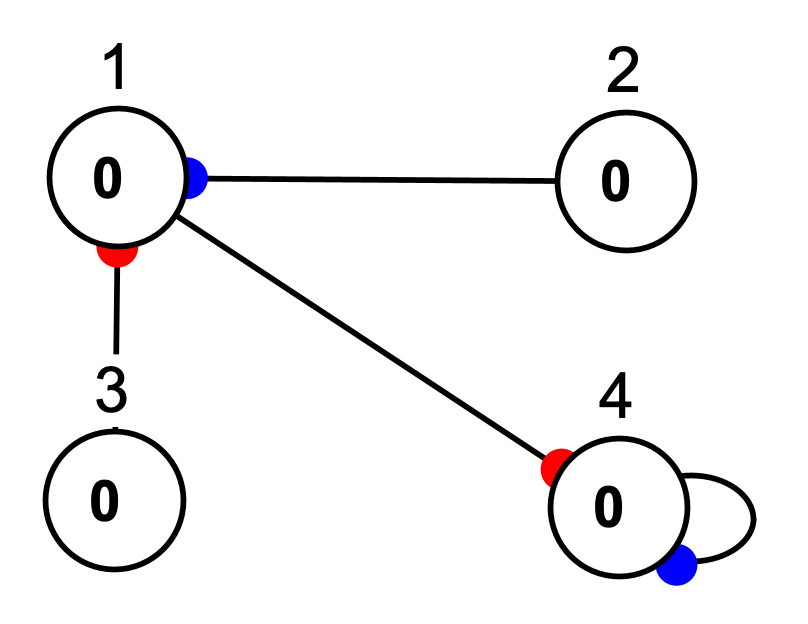
\includegraphics[scale=0.5]{./images/sparseRecurrent.png}
\caption[Jeff Yoshimi.]{A sparse recurrent network, where most of the possible connections do not exist, so that in its matrix representation most entries will be 0. In this network red weights have a strength of 1 and blue weights have a strength of -1.} 
\label{sparseRecurrent}
\end{figure}

Figure \ref{sparseRecurrent} shows another example, that shows what we do when some links are missing. If a weight does not exist, it is represented by a $0$ in the corresponding matrix. Here is its representation:

% Make this a table with a caption but keep this position
\begin{minipage}{0.5\textwidth}
\centering
\[
\begin{array}{|c|c|c|c|c|}
\hline
\multicolumn{1}{|c|}{} & \textbf{1} & \textbf{2}  & \textbf{3} & \textbf{4} \\
\hline
\textbf{1} & 0 & 0 & 0 & 1 \\
\hline
\textbf{2} & -1 & 0 & 0 & 0 \\
\hline
\textbf{3} & 1 & 0 & 0 & 0 \\
\hline
\textbf{4} & 0 & 0 & 0 & -1 \\
\hline
\end{array}
\]
\end{minipage}
\begin{minipage}{0.5\textwidth}
\centering
\[
\begin{pmatrix}
0 & 0 & 0 & 1 \\
-1 & 0 & 0 & 0 \\
1 & 0 & 0 & 0 \\
0 & 0 & 0 & -1
\end{pmatrix}
\]
\end{minipage}
\vspace*{.1cm} 

\noindent Now let's check your understanding: there are 4 nodes and thus the matrix is 4-by-4. There are two positive weights and two negative weights, and there are two positive entries and two negative entries in the table. Node 4 is self-connected and the fourth diagonal entry is non-zero. Nodes 1 and 4 have two weights in their fan-in and those two columns have two entries.

% Change refs below to refs to the table
In the special case where most of the entries in a weight matrix are $0$, the matrix is called a \glossary{sparse matrix}. The matrix representing the weights in figure \ref{sparseRecurrent} is sparse. A sparse matrix is contrasted with dense matrix, where most of the entries are non-zero. Really these are two ends of a continuum described by a number called \glossary{sparsity}, which ranges from $0$ to $1$, and where higher values are more sparse. The sparsity of a matrix is obtained by counting how many zero entries the matrix has and dividing by the total number of entries. If all of the matrix entries are $0$ then the sparsity of the matrix is $1$. If half of the entries are $0$ then the sparsity is $.5$.  If none of the matrix entries are $0$ then the sparsity of the matrix is $0$. The matrix in the table above has $16$ entries, $12$ of which are $0$, so its sparsity is $12/16 = 3/4 = .75$. Sparse weight matrices represent sparsely connected networks, where only a few of the possible connections between relevant nodes exist (recall that a matrix representation of a network uses $0$ to represent the absence of a connection).  Dense matrices are used to represent densely connected networks. The word ``dense connection'' or ``dense weight layer'' in this context often implies a sparsity of $0$, that is, an ``all-to-all'' or ``fully connected'' set of weights between relevant nodes.
% Think about whether some clarification about feed-forward and recurrent weight layers is needed


\section{Graphical Conventions}\label{sourceTarget} 

% Simbrain 4 images. Settle the issue in Simbrain first then add the images here and in the next section. And note that the image can be set up to display either way.

% See "by hand" lectures Tom Yeh.
% Nice pics and walk through here: https://e2eml.school/transformers.html
% To get to the next belt level, you have to deal with this kind of thing, and so train your brain to deal with it.
% Note there are other reps too, like the points in a space rep.

At this point we take a break to prepare for thinking graphically about the matrix product. We are going to start thinking more about matrices as ways of transforming vectors, of channeling information from one layer of a network to another.\footnote{In fact, the book as a whole can be thought of as involving two tracks: a `scalar' and a `vectorized' track. We use vectors and matrices to understand many ideas conceptually, but we do not make heavy use of matrix products or matrix algebra. This is much more accessible at first and supports a main thread in the book and Simbrain, making neural networks easy enough to use without any math background at all (there is math to learn, but it is self contained). However, this is not how things are done by most professionals working on neural networks in industry, and most academics as well. For any serious work, we must move to a more vectorized approach. Everything becomes more concise, and runs more efficiently on high-performance computers. This requires a change in thinking, a way of seeing and thinking about these problems in terms of matrices, vectors, and tensors, often seeing datasets and batches in new ways. The focus here is on vectors, matrices, and higher rank tensors, and on applying linear algebra methods directly to these structures.} We will, in particular, be focusing on  the matrix product, or matrix multiplication. This operation (and its generalization, the tensor product), are at the heart of a great deal of the mathematics of neural networks. However, it is not an easy operation to master, because various entries must be held in memory, multiplied and added, and then ``written out'' in a specific way.  it's quite easy to lose track.  Moreover, we'd like to stay within the visual framework of Simbrain and find ways to quickly and intuitively understand what is going on. For that purpose we will begin to move from the ball and stick metaphors we have emphasized to one that shows matrices directly, and we need to have an ability to visualize how information flows through these structures.

Fortunately there are ways to simplify the process. We will see that the only basic visualization we need is one where we think about vectors being transformed through matrices, or ``flowing'' through matrices.  Later when we consider matrices or tensors being transformed, we can use the same exact mental models, because we can think of these as cases where a bunch of vectors are all arranged in rows or columns, and processed one at a time. For example, we will often consider ``stacks'' of vectors and how they are processed by matrices.  Think of the matrices as static processors and as the tensors that pass through them as collections of vectors that are processed one at a time.

We have already alluded above to the fact that there can be multiple ways to represent a weight matrix. For most of the book, we simply default to a ``source-target'' representation, but a target-source representation is also possible, and in many contexts is more common. If you don't care about the details, you can skip the next paragraph and just focus on the source-target representation.

% We also call this a  $\textbf{W}_{i, j}$ rep vs a  $\textbf{W}_{j,i}$.
In a ``source-target'' representation, a weight $w_{i, j}$ is a weight from source neuron $i$ to target neuron $j$. In the corresponding matrix, rows are associated with source neurons and columns are associated with target neurons. This kind of indexing is easy and natural to think about' it's what Don Norman calls a ``natural affordance'', since we are going from a source to a target.  By contrast,  a ``target-source'' format is one where we swap indices so that weight $w_{j, i}$ shows the target neuron first and the source neuron second.  In the corresponding matrix, rows are associated with target neurons and columns are associated with source neurons. This seems backwards, but for certain matrix operations is more natural and more compact to write, and so it is commonly used.\footnote{There is some disciplinary variance on which representation to use. According to wikipedia, ``The [source-target] definition is commonly used in graph theory and social network analysis (e.g., sociology, political science, economics, psychology). The [target-vector representation] is more common in other applied sciences (e.g., dynamical systems, physics, network science) where A is sometimes used to describe linear dynamics on graphs'' \url{https://en.wikipedia.org/wiki/Adjacency_matrix\#Directed_graphs}.}
% Yet another option is (from, to) vs (to, from). 

We now consider graphical conventions. We need to bridge between the ball-and-stick models we have been using and direct representations of weight matrices and activation vectors. We need a template for mentally moving back and forth between these ways of thinking. One byproduct of preparing this way of thinking is that it will be easy for us to see how a matrix can take us from one size space to another, sometimes ``down projecting'', sometimes ``up projecting'', and sometimes transforming vectors in the same-sized space.

In each case below, this is a \emph{suggested} way of thinking about the matrix, a convention.  A particular set of flow lines is shown.  One important idea to be aware of us that within each convention, we can go either forward through the flow lines in the way shown, or \emph{backwards} through them, which is what happens in backprop (chapter \extref{ch_lms_backprop}).  Whether we go forward or backward depends on whether we use right or left multiplication, which is a topic taken up in the next section.

\subsection{Source-target graphical conventions}

Figure \ref{sourceTargetConvention} shows how to think of a matrix in source-target format as channeling information.  We can think of the number of rows $m$ as corresponding to the number of inputs, and the number of columns $n$ as corresponding to the number of outputs.  Then for example, a $2x3$ matrix takes us from 2 inputs to 3 outputs. This is naturally represented by a ``left multiplication'', as we will see below. We can still multiply the other way, but in the other case we are moving ``backwards'' through the matrix (which is actually done in backprop).  What is shown here is a matrix that takes us from a 2 dimensional to a 3 dimensional space, which is a \glossary{up projection}.  If it were a $3x2$ matrix it would take us from a three dimensional space to a 2 dimensional space, a \glossary{down projection}. If it were a $2x2$ matrix it would transform things in the same 2 dimensional space.

\begin{figure}[h]
\centering
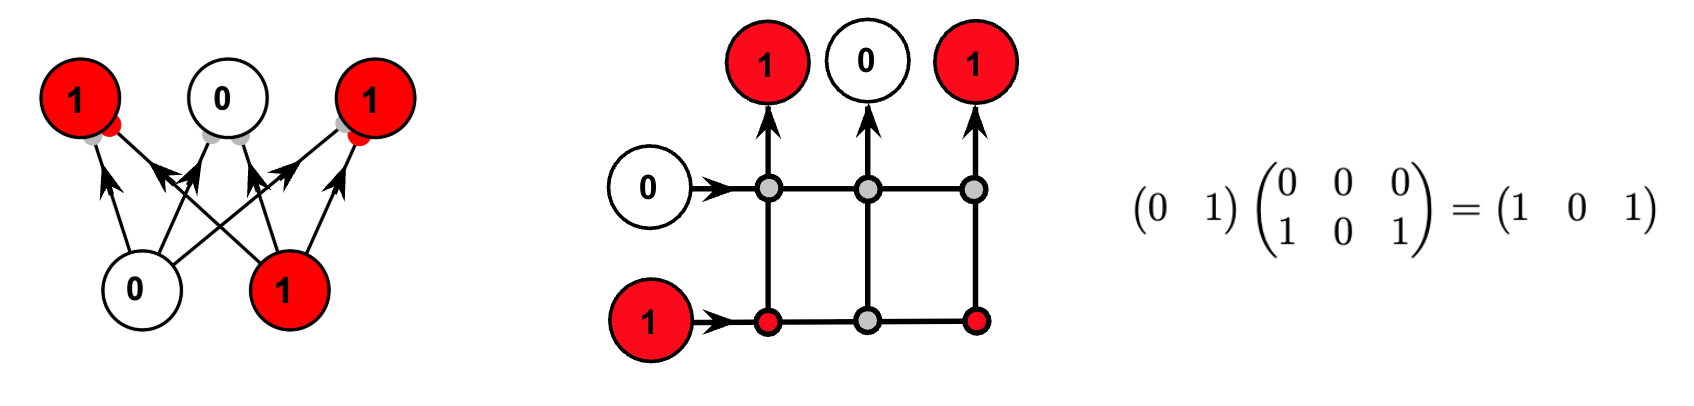
\includegraphics[width=0.75\textwidth]{images/sourceTarget.png}
\caption[Jeff Yoshimi.]{Graphical model for thinking about a weight matrix using a source-target representation. We think of the vectors as entering the matrix on the left, being multiplied and added, and exiting up top.}
\label{sourceTargetConvention}
\end{figure}

Figure \ref{sourceTargetSimbrain} shows how this looks in Simbrain. You are encouraged to imagine  the input activations being rotated and ``entering'' on the left (in Simbrain, you can also rotate the presentation of the input vector), and then ``exiting'' above.  Depending on how you set things up in Simbrain you will have to imagine the input and output rotating and moving in various ways (in this example, the input must rotate and the output must move over to the right), but in general just set things up mentally to enter on the left and exist above, and you should be able to interpret what is happening.

\begin{figure}[h]
\centering
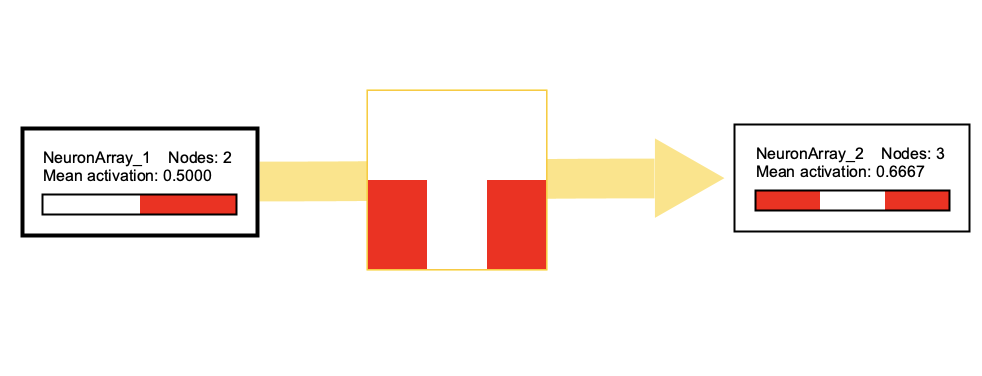
\includegraphics[width=0.5\textwidth]{images/sourceTargetSimbrain.png}
\caption[Jeff Yoshimi.]{Using a source-target representation in Simbrain. We think of the vectors as entering the matrix on the left and exiting up top.}
\label{sourceTargetSimbrain}
\end{figure}

\subsection{Target-source graphical conventions}

Figure \ref{targetSourceConvention} shows how to think of a matrix in target-source format as channeling information.  We can think of the number of rows $m$ as corresponding to the number of outputs, and the number of columns $n$ as corresponding to the number of inputs. This is the exact same situation as above, but the different order of the indices creates a different shape for the matrix, and so we  think about things in this alternative way.  

\begin{figure}[h]
\centering
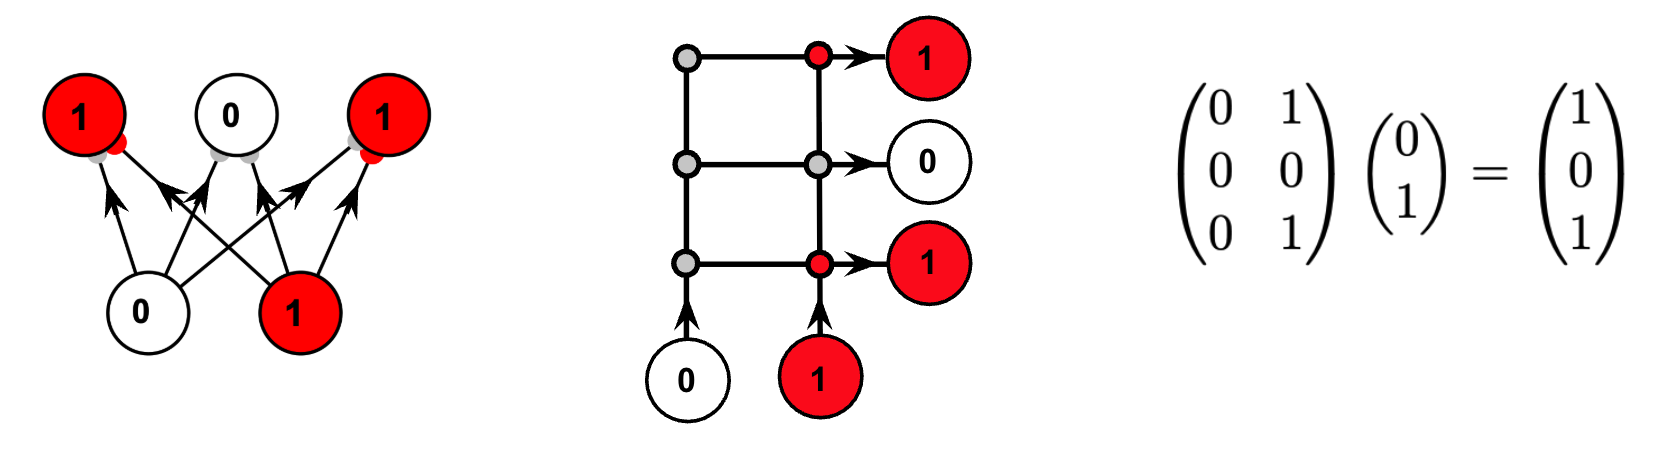
\includegraphics[width=0.75\textwidth]{images/targetSource.png}
\caption[Jeff Yoshimi.]{Graphical model for thinking about a weight matrix using a target-source representation. We think of the vectors as entering the matrix from below, being multiplied and added, and exiting to the right. }
\label{targetSourceConvention}
\end{figure}

Figure \ref{targetSourceSimbrain} shows how this configuration looks in Simbrain. Here you are encouraged to imagine  the input activations  ``entering'' from below and then ``exiting'' to the right.

\begin{figure}[h]
\centering
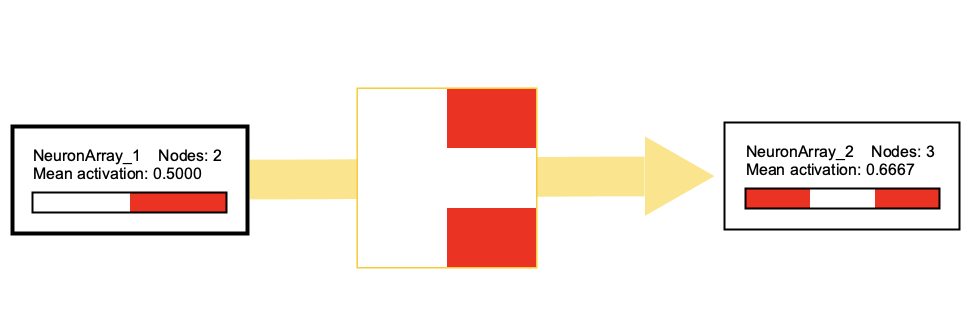
\includegraphics[width=0.5\textwidth]{images/targetSourceSimbrain.png}
\caption[Jeff Yoshimi.]{Using a target-source representation in Simbrain. We think of the vectors as entering the matrix from below and exiting to the right.}
\label{targetSourceSimbrain}
\end{figure}

\section{Matrix Multiplication (Part 1)}

In this section we begin a discussion of matrix multiplication, where two matrices are multiplied by one another. There is nothing fundamentally difficult about this operation: it is just a combination of multiplying and adding entries, but the details can be tricky. There are established conventions for which things to multiply and add together, and they can be hard to remember. However, being able to do these computations is a crucial skill in neural networks, given how pervasive they are. Adding to the difficulty is that there is a kind of ambiguity to the process: matrix multiplications can often be thought of in different but compatible ways, as we will see.

We start with the case where one of the matrices is a vector (recall that vectors are a kind of matrix, where there is either a single row or a single column). When a matrix is multiplied by a column vector it is called left multiplication (because the matrix is on the left). When a row vector is multiplied by a matrix it is called right multiplication (because the matrix is on the right). In the first case of $\mathbf{A}v$ we go from matrix and column vector to a new column vector. In the second case of $v\mathbf{A}$ we go from a row vector and a matrix to a new row vector.  The first case ``processes'' an input row into a transformed output row. The second case processes an input column vector into a transformed column vector (this concept of ``processing'' will be important below). These cases are good to start with because they show the basic mechanics of the operations, which is to take a vector, and ``scan'' it over the matrix in a certain way, taking dot products as you do, which are then ``written out'' to an output vector.  

Even though left multiplication is a bit more common in math, we start with right multiplication because it is a more natural starting place with the source-target graphical structure we've been emphasizing.  With a source-target scheme a  ``forward pass'' through a matrix is corresponds to a right multiplication, and backward pass (as in backprop) corresponds to a left multiplication. (In a target-source scheme this is reversed. A forward pass correspond to left multiplication and a backward pass corresponds to right multiplication).

With right multiplication we start with a row vector and multiply it by a matrix on the right. We take the dot product of the row vector and the first column vector in the matrix (see figure \ref{vectorMatrixProduct}. The resulting number is the first component of a row vector. Then do this for each of the remaining columns of the matrix, adding these dot products to the row vector as you go. The resulting row vector is the matrix product of a row vector and a matrix. Intuitively, it is like you are writing out the matrix product, one number at a time, by dotting the vector on the right with each of the columns of the weight matrix.  In a sense we have transformed one row vector into another. The matrix represents the transformation, the row vector on the left is the input, and the row vector on the left is the output (the analogy to neural networks should be clear).\footnote{The idea that a matrix represents a way of transforming vectors is common in mathematics. In fact, matrices are often used to represent linear transformations, where one vector is converted in to another using a linear function. Think of a set of points in the plane (vectors in a 2 dimensional space) getting moved in some specific way. The way these points move can be represented, in some cases, by multiplying each point by a matrix. For example, when you use a drawing program to modify a simple line graphic (a bunch of points in a plane) the transformation of the selected set of points is implemented using matrix multiplication. Rotations about the origin, reflections about a line through the origin, and dilations and contractions about the origin are linear transformations.}

\begin{figure}[h]
\centering
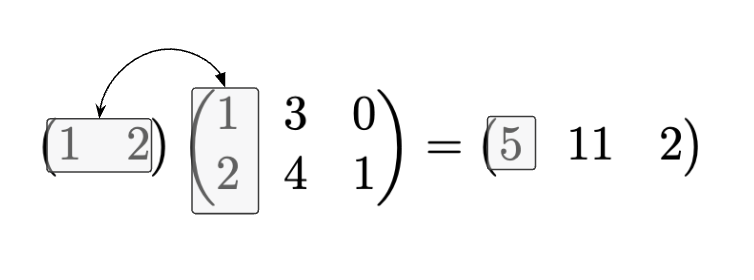
\includegraphics[width=0.4\textwidth]{images/vectorMatrixProduct.png}
\caption[Jeff Yoshimi.]{The row vector can be thought of as being rotated and scanned along the matrix to its right, writing out the output vector, which is also a row vector. Alternatively the columns of the matrix can be thought of as being removed one by one and dotted with the row vector, writing out the output vector.}
\label{vectorMatrixProduct}
\end{figure}

Here's the example from figure \ref{vectorMatrixProduct} worked out:
\[
  \begin{matrix}\begin{pmatrix}1 & 2\end{pmatrix}\\\mbox{}\end{matrix}
  \begin{pmatrix} 1 & 3 & 0 \\ 2 & 4 & 1 \end{pmatrix} 
  =
  \bigg( (1)(1) + (2)(2) ,\;\; (1)(3) + (2)(4) ,\;\; (1)(0)+ (2)(1) \bigg)
  =
  \begin{pmatrix}  5 \;\; 11 \;\;\; 2  \end{pmatrix}
\]
\vspace*{.1cm} 

So in this case row vectors are transformed into row vectors. This approach is less common in math, perhaps because it takes more space to write out. However, we will see a variant on this approach is quite common when we deal with larger matrix products.

The same example can also be represented by a right multiplication, where we transpose the matrix (see appendix for a definition of transpose). With left multiplication  a matrix on the left is multiplied by a column vector to produce a new column vector. We can think of the matrix as ``operating'' on the vector. Figure \ref{matrixVectorProduct} shows how to perform the operation. Take the column vector and dot it with the first row to produce a the first entry in the output column vector. Then scan down the rows the write out the result.  In a sense we have transformed the vector. The matrix represents the transformation, the vector on the right of the matrix is the input, and the vector after the equals sign is the output (the analogy to neural networks should be clear).

\begin{figure}[h]
\centering
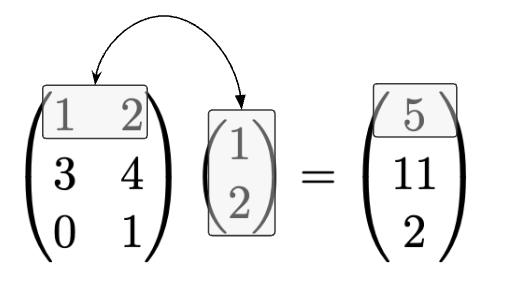
\includegraphics[width=0.5\textwidth]{images/matrixVectorProduct.png}
\caption[Jeff Yoshimi.]{The column vector can be thought of as being mental rotated and scanned across the rows of the matrix to it's left, taking dot products along the way which are written out to the output vector, which is also a column vector. Alternatively, think of removing the rows from the matrix one by one, and dotting with the column vector, writing out the output vector as we do.}
\label{matrixVectorProduct}
\end{figure}

Here's the example from Figure \ref{matrixVectorProduct} worked out:
\[
  \begin{pmatrix}
    1 & 2 \\
    3 & 4 \\
    0 & 1
  \end{pmatrix}
    \begin{matrix}
    \begin{pmatrix}1\\2\end{pmatrix}
  \end{matrix}
  =
  \begin{pmatrix}
    (1)(1) + (2)(2) \\
    (1)(3) + (2)(4) \\
    (1)(0) + (2)(1)
  \end{pmatrix}
  =
  \begin{pmatrix}
    5 \\
    11 \\
    2
  \end{pmatrix}
\]
\vspace*{.1cm}


So we have seen that the very same operation can be represented in two equivalent ways, by using the transpose. This is based on the theorem that  $\mathbf{A}v =  v^T\mathbf{A}^T$, and is the basis of the ambiguity mentioned above. 

\section{Matrix Multiplication (Applications)}

% We will introduce some graphical conventions here. There will be variants on them throughout the book.

In this section we apply the ideas above, focus on the case of a row vector times a matrix.\footnote{This matches the source-target format for representing fan-in weight vectors (see section \ref{sourceTarget}) which we have chosen for convenience in much of this book.} In this way we produce a new output vector. Each of these dot products is a weighted input (see chapter \extref{ch_act_functions}). Assuming a default unbounded linear activation function, this can be used to represent weight propagation. We consider the feed-forward case first, then the recurrent case.

Consider the feed-forward network in figure \ref{labelledNets}, which uses linear activation functions without bias (we are also ignoring clipping) so that node activations just are weighted inputs. That is, we multiply the input vector by the intervening weight matrix to obtain the hidden unit vector:  $\textbf{a}_{hidden} = \textbf{a}_{input} \textbf{W}_{input,hidden}$. We can then multiply the hidden unit vector by the hidden-to-output layer weight matrix to get the output vector. We can continue to do this for all the layers of a feed-forward network. So, for linear networks, pretty much all we do when updating the network is use matrix products (and even for non-linear networks, we use the matrix product to compute vectors of weighted inputs, which are then transformed by, for example, sigmoid functions).

Suppose the feed-forward network in figure \ref{labelledNets} has linear activation functions and 0 bias, and its input activation vector is $\textbf{a}_{input} = (1,2)$. To compute the hidden layer activation vector, we compute the dot product between the input vector and each of the three column vectors:
\[
  \begin{matrix}\begin{pmatrix}1 & 2\end{pmatrix}\\\mbox{}\end{matrix}
  \begin{pmatrix} 1 & 0.7 & 2 \\ -2 & -1 & 2.1 \end{pmatrix} 
  =
  \bigg( (1)(1) + (2)(-2) ,\;\; (1)(0.7) + (2)(-1) ,\;\; (1)(2)+ (2)(2.1) \bigg)
  =
  \begin{pmatrix}  -3 \;\; -1.3 \;\;\; 6.2  \end{pmatrix}
\]
\vspace*{.1cm} 

This can be visualized by imagining that an input activation vector is being combined (``dotted'') with the fan-in weight vectors of each of the three nodes at the next layer, to produce the weighted input to each of them and thus the next layer's activation vector. 

% 1,2 as input confusing because it overlaps indices in video. Change?
Now for the recurrent case. We can do the same kind of thing with the sparse recurrent network in figure \ref{sparseRecurrent}, but in this case we will be determining its activations at successive time steps. This is because with a recurrent network, the output can always be fed right back into the network as input, which gives these networks their dynamic properties. Let the weight matrix be  $\textbf{W}_{r}$ then a sequence of activation vectors $\textbf{a}(1), \textbf{a}(2), \textbf{a}(3), \dots$ (with time in parentheses) is given by $\textbf{a}(2) = \textbf{a}(1) \textbf{W}_{r}$, $\textbf{a}(3) = \textbf{a}(2) \textbf{W}_{r}$, etc. 

This is easy to see by examples. Suppose we have activated node 2 of the network in figure \ref{sparseRecurrent} and we start iterating. Since the activations and weights are all whole numbers, it's not too hard to compute this out for a few time steps. Again just dot the input vector by the columns to write out the first output, where we get the activation vector at time 2 by multiplying the initial activation vector by the weight matrix (that is, $\textbf{a}(1) \textbf{W}_{r} = \textbf{a}(2)$):
\[
\begin{pmatrix}
0 & 1 & 0 & 0  
\end{pmatrix} 
\begin{pmatrix}
0 & 0 & 0 & 1 \\
-1 & 0 & 0 & 0 \\
1 & 0 & 0 & 0 \\
0 & 0 & 0 & -1
\end{pmatrix}
=
\begin{pmatrix}
-1 & 0 & 0 & 0
\end{pmatrix} 
\]
\vspace*{.1cm} 

\noindent Try to do it in your head, dotting the $(-1, 0,0,0)$ with the four columns of the matrix and thereby writing out the output vector. In the next iteration you will get $(0,0,0,-1)$, then $(0,0,0,1)$. If we keep going we get the following sequence of states from the initial state $(0,1,0,0$):
\begin{equation*}
(0,1,0,0),\; (-1,0,0,0),\; (0,0,0,-1),\; (0,0,0,1),\;  (0,0,0,-1)\; \dots
\end{equation*}
You can easily set this up in Simbrain and confirm this is what happens. We will see in the dynamical systems chapter \extref{ch_dst} that this is one \emph{orbit} in the network's activation space. In this case, the network has started to oscillate between two states, and it will do that forever, and that behavior is basically encoded in the weight matrix.

\section{Matrix Multiplication (Part 2)}\label{matrixMultiplication}

% This is awesome but fork it and do it my way: http://matrixmultiplication.xyz/

We now consider arbitrary matrix multiplications, rather than cases where one of the matrices is a vector. However, we make use of mental models we developed in the matrix/vector case.

Consider a matrix multiplication 
\begin{align*}
\mathbf{A}\mathbf{B} = \mathbf{C}
\end{align*}

% Need lots of new exercises 
A first useful skill to have down before getting to computations is the skill of checking to see that a matrix multiplication is possible, and also anticipating what the shape of the output will be. This is nice and easy to do. If $\mathbf{A}$ has shape $(m, n)$ and matrix $\mathbf{B}$ has shape $(n, p)$, then the product $\mathbf{C}$ is defined and has shape $(m, p)$. For example: 
\[
\text{Shape: } (5 \times 2) \times (2 \times 7) \Rightarrow (5 \times 7)
\]
The ``inner'' dimensions (2 and 2) match, so the multiplication is valid. The resulting matrix is $5 \times 7$. Notice that as long as the inner dimensions match, we can have any ``outer'' dimensions we like. 
% Some matrices will take us from a lower dimension to a higher dimensional space (these are sometimes called ``up projections'').  Other matrices will take us from a higher dimensional space to a lower dimensional space (these are sometimes called ``down projections'') 

A multiplication $\mathbf{A}\mathbf{B} = \mathbf{C}$ can be interpreted in several complementary ways. Perhaps the most common way is ``entrywise'': the $(i,j)$ entry of the result $\mathbf{C}$ is computed by taking the dot product of the $i$th row of $\mathbf{A}$ and the $j$th column of $\mathbf{B}$. See figure \ref{entryWiseMatrixProduct} for an illustration. 

\begin{figure}[h]
\centering
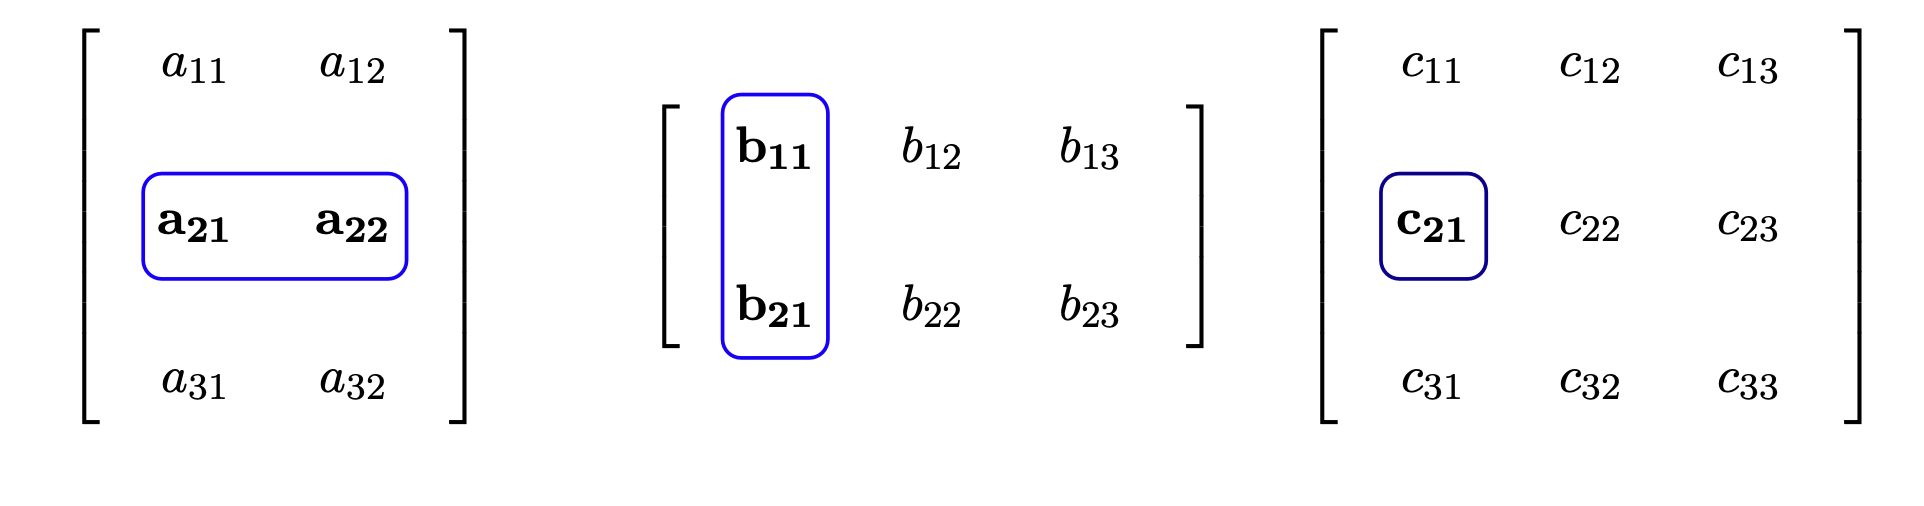
\includegraphics[width=0.5\textwidth]{images/matrixProductEntryWise.png}
\caption[Jeff Yoshimi.]{Row $i$, column $j$ of $\mathbf{C}$ is the dot product of row $i$ of $\mathbf{A}$ and column $j$ of $\mathbf{B}$. Here entry $(2,1)$ of $\mathbf{C}$ is the dot product of row $2$ of $\mathbf{A}$ and column $1$ of $\mathbf{B}$.}
\label{entryWiseMatrixProduct}
\end{figure}

However, often when dealing with neural network applications, it helps to zoom-out and imagine that rows or columns are being ``processed'' by the matrix. This builds on the idea left multiplications transforms columns to new columns and that right multiplication transforms rows to new rows. In the more general case, it turns out the row to row perspective is helpful and perhaps more common in some discussions. 

We will start with the ``row processing'' respective. Here we view $\mathbf{A}$ in  $\mathbf{A}\mathbf{B} = \mathbf{C}$ as a stack of row vectors which we peel off one by one and right multiply by $\mathbf{B}$ to build up $\mathbf{C}$.\footnote{Alternatively, we can think of this as taking linear combinations of the rows of $\mathbf{B}$, which is another useful perspective.} This idea of taking a stack of rows and pushing them through a matrix to get another stack of rows is common with batch processing and in understanding how representations ``move'' through a transformer.\footnote{See \url{ https://e2eml.school/transformers.html}.}

Figure \ref{rowPerspective} shows the idea abstractly. We peel off the rows of $\mathbf{A}$ and multiply them by the matrix $\mathbf{B}$ as described in the discussion above. Notice that the result is another collection of rows in $\mathbf{C}$, with as many rows as were in $\mathbf{A}$, where we just think of each rows as being the matrix transformation of that row by $\mathbf{B}$. This will be crucial in the discussions of transformers in chapter \extref{ch_transformers}. 

\begin{figure}[h]
\centering
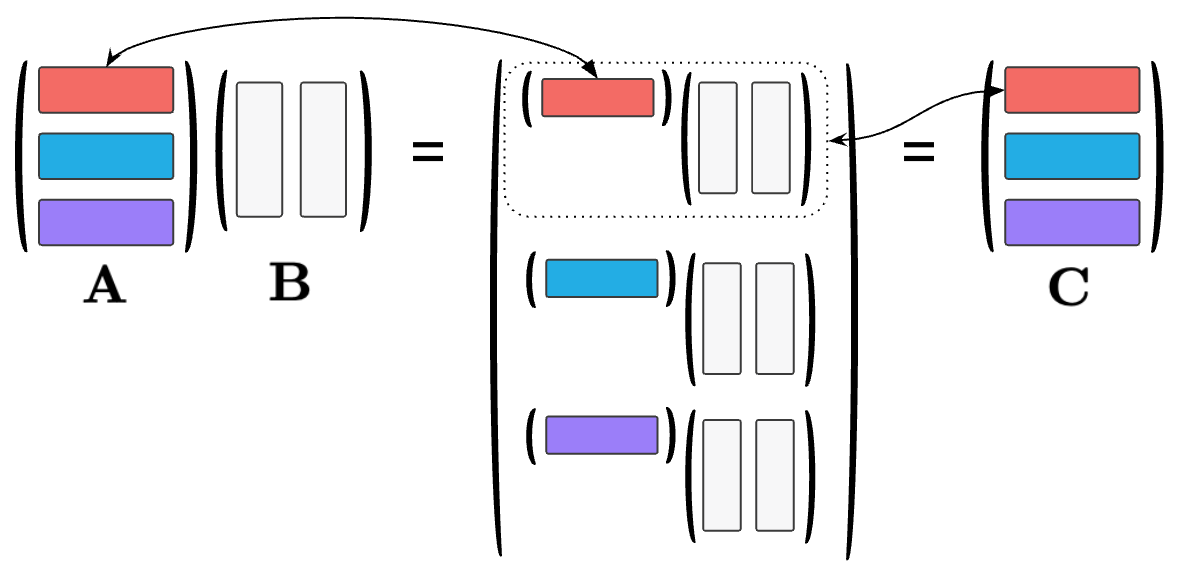
\includegraphics[width=0.5\textwidth]{images/rowPerspective.png}
\caption[Jeff Yoshimi.]{How to view a matrix multiplication  $\mathbf{A}\mathbf{B} = \mathbf{C}$ as ``row processing''.  The rows of the left matrix $\mathbf{A}$ are taken one by one, and multiplied by matrix $\mathbf{B}$  on the right, using the methods of the section above on right multiplication.  This is done for each row (as is shown in the center panel), and the end result is an output matrix $\mathbf{C}$ that can be thought of as a stack of rows, each of which has been processed by $\mathbf{B}$.}
\label{rowPerspective}
\end{figure} 

We basically repeat multiple row vector times matrix multiplications to build out the output. We think of rows of $\mathbf{A}$ as being operated on by $\mathbf{B}$:

\begin{align*}
\begin{bmatrix}
\text{--- } \mathbf{a}_1 \text{ ---} \\
\text{--- } \mathbf{a}_2 \text{ ---} \\
\vdots \\
\text{--- } \mathbf{a}_m \text{ ---}
\end{bmatrix}
\cdot
\mathbf{B}
=
\begin{bmatrix}
\text{--- } \mathbf{a}_1 \mathbf{B} \text{--- } \\
\text{--- } \mathbf{a}_2 \mathbf{B} \text{--- } \\
\vdots \\
\text{--- } \mathbf{a}_m \mathbf{B} \text{--- }
\end{bmatrix}
\end{align*}

We can also take a column perspective on generic matrix multiplications, treating $\mathbf{B}$ in $\mathbf{A}\mathbf{B} = \mathbf{C}$ as a sequence of column vectors, which we peel off one by one and left multiply by $\mathbf{A}$ to build up the columns of $\mathbf{C}$.\footnote{See \url{https://www.coursera.org/learn/matrix-algebra-determinants-and-eigenvectors/supplement/mGkyi/matrix-operations}.} 

Figure \ref{columnPerspective} shows the idea abstractly. We basically repeat multiple matrix by column vector multiplications to build out the output. 

\begin{figure}[h]
\centering
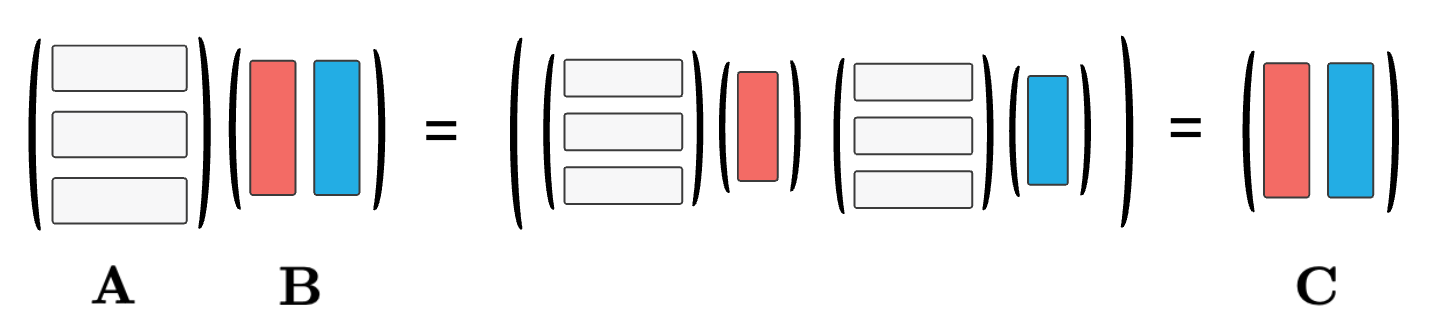
\includegraphics[width=0.6\textwidth]{images/columnPerspective.png}
\caption[Jeff Yoshimi.]{How to view a matrix multiplication  $\mathbf{A}\mathbf{B} = \mathbf{C}$ as ``column processing''.  The rows of the right matrix $\mathbf{B}$ are taken one by one, and multiplied by matrix $\mathbf{A}$  on the left, using the methods of the section above on left multiplication.  This is done for each column (as is shown in the center panel), and the end result is an output matrix $\mathbf{C}$ that can be thought of as a file of columns, each of which has been processed by $\mathbf{A}$.}
\label{columnPerspective}
\end{figure} 

We think of $\mathbf{A}$ as operating on columns of $\mathbf{B}$ to write out columns as $\mathbf{C}$:

\begin{align*}
\mathbf{A} \cdot
\begin{bmatrix}
\vert &        & \vert \\
\mathbf{b}_1 & \cdots & \mathbf{b}_n \\
\vert &        & \vert
\end{bmatrix}
=
\begin{bmatrix}
\vert &        & \vert \\
\mathbf{A} \mathbf{b}_1 & \cdots & \mathbf{A} \mathbf{b}_n \\
\vert &        & \vert
\end{bmatrix}
\end{align*}


\section{Flow Diagrams}\label{flowDiagrams}

We saw in the last section that a matrix multiplication where we think of the left matrix as a stack of rows can be thought of as transforming each row by the matrix on the right.  The output matrix has the same number of rows as the input matrix, and matrix is like a transformation operating down the rows (again, we can also do this from a column perspective, but rows are more common in the relevant contexts and so we simply decide to focus on them). 

This sets up a kind of diagram that we will sometimes use in later chapters, one where we only show the matrices and other transformations, and simply assume that stacks of rows (or other more complicated structures, like tensors, discussed next) are being processed by weight matrices, activation functions, and other mathematical operations. What we have called ``node layers'' are not shown.  One might call these matrix flow diagrams, tensor flow diagrams, activation processing diagrams, etc. There is no settled terminology to our knowledge, but this way of viewing things has become standard in the literature.

Figure \ref{flowPerspective} shows the idea. In the left panel, a matrix is shown as a stack of rows being processed by two weight matrices $\mathbf{M1}$ and $\mathbf{M2}$. This could represent a 2 weight layer feed-forward network. Notice that it's the same kind of network we talk about elsewhere in the book, but that we now think of it as processing stacks of vectors, not individual vectors. Also note the shape changes between the two matrices, in the hidden layer (a stack of hidden layer activations), but that the number of rows has stayed the same. Also notice that the bottom to rows remain zeros throughout, and so when they are multiplied by the matrices they stay zero. 

Also shown is an arrow from the input to the output, representing skip connection or residual connection. This implies that the input matrix is added to the output matrix. Addition of matrices (and other tensors, as discussed below) is defined when their shape stays the same. 

\begin{figure}[h]
\centering
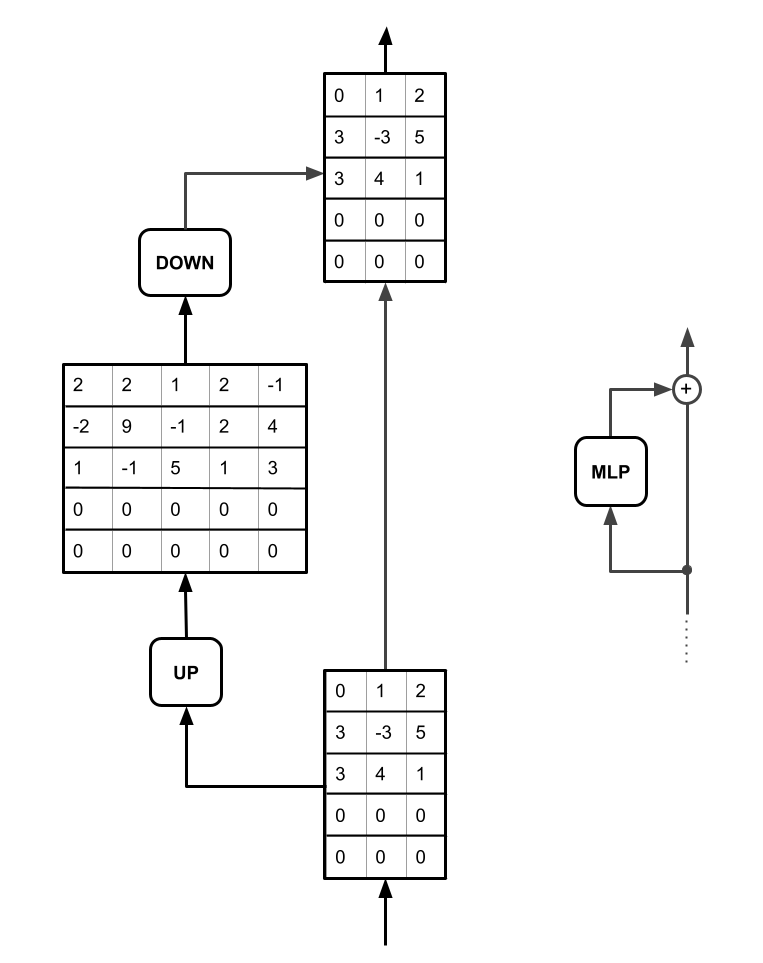
\includegraphics[width=0.3\textwidth]{images/flowPerspective.png}
\caption[Jeff Yoshimi.]{(Left panel) Two matrices are used to process a matrix input conceptualized as a stack of rows. This is essentially a two weight layer feedforward linear network, though we can assume activation functions are being applied (such as ReLU, in which case such a network might be called an ``MLP'', for multilayer perceptron. Even though it is a standard network, we can see here that it can process matrices because of the features of matrix multiplication discussed above. In this example there is also a skip or residual connection from the input to the output, which assumes that the input and output retain the same shape, even if the hidden layer activations are of a different shape. (Right panel). The entire diagram can be simplified to a simpler diagram in which only the flow of activation is shown, as well as any mathematical operations. Here the entire MLP is being reduced to a single box labeled  $\mathbf{T}$. }
\label{flowPerspective}
\end{figure} 

Overall we think of the matrices shown in bold ($\mathbf{M1}$ and $\mathbf{M2}$) as doing the processing (mainly weight matrices and related structures in this book), and of the other matrices as being processed (mainly representing stacks of activation vectors in this book).  This facilitates another kind of diagram, where we don't show the stacks of activation vectors, but only the processing elements, sometimes collapsing several processing layers into one box.  On the right of figure \ref{flowPerspective} such a diagram is shown. In this diagram the skip connection is shown as a straight line up--what is sometimes called a ``residual stream'', with the detour into a few layers of feed-forward processing shown by a box labeled $\mathbf{T}$. It's as if the processor reads from the main line then writes back to it. In this way we can have many different operations of reading to and writing from a residual stream. This will be important in the discussion of transformers and their mechanistic interpretation.
% Citations
% All components of a transformer (the token embedding, attention heads, MLP layers, and unembedding) communicate with each other by reading and writing to different subspaces of the residual stream. Rather than analyze the residual stream vectors, it can be helpful to decompose the residual stream into all these different communication channels, corresponding to paths through the model. > \cite{elhage2021mathematical}

\section{Tensors}\label{sect_tensors}

% https://stanford.edu/~shervine/teaching/cs-230/cheatsheet-convolutional-neural-networks

A \glossary{tensor} is a generalization of the concept of a vector that encompasses numbers, arrays of numbers, matrices (2d arrays of numbers), arrays of matrices, arrays of these arrays, etc. These more complex structures are increasingly common since the time of the deep learning revolution (section \extref{deep_revolution}). The basic idea is not just to work with vectors and matrices, but also sets of matrices and even sets of sets of matrices. These have special nomenclature like ``volume''. In this section we cover the basics.

% TODO: Glossary items for textbfs
% Array vs. set.  Array implies ordering. Comp sci version of tuple.
% Tensor is more math language. Ndarray is more from languages like numpy and torch
The \textbf{rank} of a  tensor is the number of indices required to specify an entry in it.These are also sometimes called ``n-dimensional arrays'' or ``n-d arrays'' (1d array, 2d array, etc.).\footnote{Note that the dimensionalty of an array is the literal dimension of the object, like a vector is 1d and a matrix is 2d. This is not the same as the dimensionality of the space these objects live in. For example, $(1,2,1,0)$ is a point in a 4d space, but it is a 1d tensor or 1d array of numbers.} The \textbf{shape} of a tensor is the number of components it has along each of the array's dimensions. We have seen this with matrices, where the shape is stated in terms of rows and columns, e.g. a $5 \times 2$ matrix. For more complex tensors the shape is specified by a number of components for each dimension of the array, like a $4 \times 2 \times 5$ volume. Here are the main types of tensor:

\begin{itemize}
\item A \textbf{scalar} is a rank 0 tensor or 0d array because it requires no indices. The number 42 is a rank 0 tensor, a 0d array, but nobody talks about it that way. 
\item A \textbf{vector} is a rank 1 tensor or 1d array because it takes one index to specify an entry in a vector, and the result is spread out in one dimension. The vector $(0,1,0)$ is a rank 1 tensor, because it takes one index to specify entries, but people usually just call it a vector. Vectors were discussed in much of this chapter, starting in section \ref{sect_vector}.
\item A \textbf{matrix} is a rank 2 tensor or 2d array, because it takes two numbers to specify an entry (a row and column index), and the result is spread out in two dimensions. We've seen lots of examples of matrices in this chapter, and they were discussed in section \ref{sect_matrices}.
\item A \textbf{volume} is an array of matrices. It is a rank 3 tensor or 3d array, because it takes 3 indices to specify an entry, and the result is spread out in three dimensions. The term ``volume'' is common but not completely standard, but is intuitive so we adopt it here. It can be visualized as a stack of matrices, or as a solid, something like a Rubik's cube or 3d chess board (see figure \ref{tensorVisualStyles}). A common use of volumes is to represent images, which requires several channels of 2d information, several ``copies'' of a pixel array. For example, an RGB color image that is 28 rows (height) by 28 columns (width) is represented by three matrices (red, green, and blue) of shape $28 \times 28$. Thus the whole image is represented by a tensor with shape $3 \times 28 \times 28$.  These indices are referred to as depth or channel, width, and height. 
\item A \textbf{batch of volumes} is an array of volumes. It is a rank 4 tensor or 4d array because it takes 4 indices to specify an entry. It is spread out in four dimensions, but since we can't visualize that we can instead visualize a set of volumes, as in the right panel of figure \ref{tensorTypes}. The word ``batch'' is used here because we are often dealing with sets or batches of inputs in a training dataset (see chapter \extref{ch_data_science}), in this case batches of RGB images, each of which is a volume with 3 channels. For example, if the images are $3 \times 28 \times 28$, then the batch of 100 images has shape $100 \times 3 \times 28 \times 28$. 
\end{itemize}

 % Rank 5 tensor examples: batch size x time steps x height x width x channels. Brain scan. Each brain scan is 3d and it's color so there are channels. So a batch of those.

Examples of each of these types of tensor are shown in figure \ref{tensorTypes}. More examples are in chapter \extref{ch_cnn}.

\begin{figure}[h]
\centering
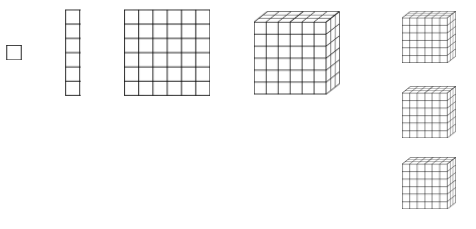
\includegraphics[scale=0.6]{./images/tensorTypes.png}
\caption[Soraya Boza.]{Schematic of different types of tensor. From left to right: a scalar, a vector, a matrix, a volume, and a batch of volumes. It can be seen that they are 0d, 1d, 2d, 3d and 4d arrays.  Numbers are not drawn in; only the abstract shape of the tensors are shown.} 
\label{tensorTypes}
\end{figure}

\begin{figure}[h]
\centering
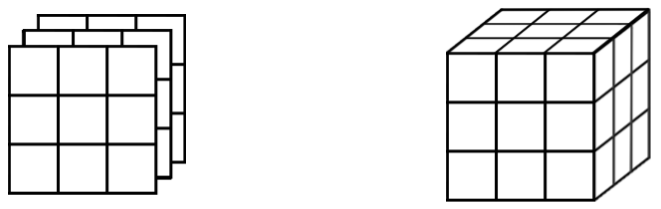
\includegraphics[scale=0.3]{./images/tensorVisualStyles.png}
\caption[Soraya Boza.]{Two ways a representing a 3d array: a stack of matrices (left) vs. a solid ``Rubik's cube''  or volume (right). Depending on the context one or the other representation is more useful.} 
\label{tensorVisualStyles}
\end{figure}

We can refer to the different indices for a tensor using standardized names in a standard order: batch size, depth (number of channels), height, and width.\footnote{This is sometimes called NCHW format (number of samples, channels, height, width). However, usage varies. Some put height and width first in indexing; some put them last in indexing. Number of channels is also ``depth'' and number of samples is also ``batch size''. Even though the rank of a tensor is the number of indices \emph{required} to specify an entry, sometimes additional entries are included (e.g. specifying a vector as a column vector assumes it is being placed in a 2d space). Thus the presentation of the ``shape'' of a tensor can vary.  In figure \ref{tensorTypes} the shapes might be given as $1 \times 1$, $6 \times 1$, $6 \times 6$, $3 \times 6 \times 6$, and $3 \times 3 \times 6 \times 6$.}
% Can use all numbers in a shape or not, depending on the context (e.g a library might require a 4 tuple to specify a tensor even if it is a vector, like 1x1x6x5).
% Much of the work in dealing with neural networks and neural net libraries is taking subsets of these tensors, slicing and indexing them, filtering them, and passing the right shaped thing from one place to another

\section{Appendix: Vector Operations}\label{S:LinearAlgebraAppendix}

% TODO: Organize into subsections?
% Add matrix operations? Like adding and subtracting same-sized matrices
% Pictures of adding and subtracting

Vectors are not just lists of numbers. They are members of \emph{vector spaces}, which are abstract mathematical spaces that have an addition operation and a scalar multiplication operation, and other operations that can be defined on the basis of these. In this appendix we introduce these two basic operations and several others. We also develop the formal definition of a vector space.
   
   The addition of two vectors with $n$ components, or \glossary{vector addition}, is simply the component-wise addition of the two vectors. This is easiest to see by example. Here is an example of adding two vectors with 3 components:
\begin{equation*}
      (\; 0,\; -1,\; 9) + (\; 1,\; 2,\; 4) 
  = (\; 0+1,\; -1+2,\; 9+4) = (1, 1, 13)
\end{equation*}
Here are a few more examples:
\begin{eqnarray*}
(1,1) + (2,3) &=& (3,4)  \\
(1,-1,1) + (0,0,0) &=& (1,-1,1)  \\
(2,3,5,8,13,21) + (3,5,8,13,21,34) &=& (5,8,13,21,34,55) \\
(-1,.5,\sqrt{7}) + (-1,-2,.8) &=& (-2,-1.5,\sqrt{7}+.8)
\end{eqnarray*}

In a similar way, \emph{vector subtraction} is the component-wise subtraction of the corresponding components of two vectors.\footnote{Vector subtraction can be defined in terms of vector addition and scalar multiplication. Thus vector subtraction is not fundamental to the definition of a vector space. It is nonetheless presented here because it is used in several other places in this book.}  Here are some examples:
\begin{eqnarray*}
(1,1,1) - (0,1,0) = (1-0,1-1,1-0) &=& (1,0,1) \\
(10,5) - (5,10) = (10-5,5-10) &=& (5,-5) \\
(1,2,3,4,5,6,7) - (0,0,0,0,0,0,0) &=& (1,2,3,4,5,6,7) \\
(2,6,1) - (.5,20,-100) &=& (1.5,-14,101)
\end{eqnarray*}

If all of the components of a vector are $0$ we call it the \glossary{zero 
vector}. Adding the zero vector to any vector leaves it unchanged.

  Another operation that can be performed with vectors is ``scalar 
multiplication''. A \glossary{scalar} is a generic term for the type of
numbers we choose to work with. These numbers are called scalars because we 
can ``rescale'' vectors using scalar multiplication. Usually we work with real 
numbers in which case we say our scalars are real numbers. Sometimes people 
use complex numbers or something even more exotic for their scalars. 

  The \glossary{scalar multiplication} of a scalar and a vector is obtained by 
multiplying each of the vectors component's by the scalar. Scalar 
multiplication is indicated by placing the scalar and vector next to each other 
without any intervening symbols. For example scalar multiplication of the 
scalar $3$ with the vector $( 1, 2, 4)$ can be written as
\begin{equation*}
3(\; 1, \; 2, \; 4) = (\; 3 \cdot 1, \; 3 \cdot 2, \; 3 \cdot 4) 
= (\; 3,\; 6, \; 12)
\end{equation*}

   The operations of vector addition and scalar multiplication can be combined.
The result is called a \glossary{linear combination} of vectors. For example
\begin{equation*}
  1 (\; 0,\; 0) + 2 (\; 0,\; 1) + 3 (\; 1,\; 0) + 4 (\; 1,\; 1) =  (\; 7,\; 6)
\end{equation*}
is a linear combination of the vectors $(0,0)$, $(0,1)$, $(1,0)$, and $(1,1)$.

   Scalar multiplication of any vector with the number $0$ is the zero vector.
The scalar multiple of a vector with the scalar $-1$ gives us the negative
of the vector. We define \glossary{vector subtraction} of one vector from 
another as the addition of the vector's negative. Subtracting a vector from 
itself is the zero vector.
\begin{eqnarray*}
  (\; 1, \; 2, \; 4) - (\; 1, \; 2, \; 4) = 
  (\; 1, \; 2, \; 4) + (\; -1, \; -2, \; -4) = (0,0,0)
\end{eqnarray*}

 Now we can more formally define a vector space. A set of vectors that satisfies two conditions
\begin{quote}
(1) The sum of any two vectors in the set is also in the set.\\
(2) Every scalar multiple of a vector in the set is also in the set. 
\end{quote}
is called a \glossary{vector space}. We will apply vector spaces to neural 
networks in chapter \extref{ch_dst}. If a subset of a vector space satisfies these 
conditions, we say it is a \glossary{subspace} of the vector space. These 
definitions allow a vector space to be a subspace of itself. 

% Scott would like to make some revisions around here
   The set of all linear combinations of a set of vectors is called the 
\glossary{span} of the vectors. The span of a set of vectors forms a 
subspace. If the span of a set of vectors is the whole vector space and any
proper subset of that set of vectors does not span the whole vector space, then 
that set of vectors is a \glossary{basis} of the vector space. There are
many different bases\footnote{``Bases'' is plural for ``basis''.} for a vector space but 
all of them have the same number of members. This number is the dimension of 
the vector space. 

   For example
\begin{eqnarray*}
\{ (1,0), (0,1) \} \quad \{ (1,2), (1,1) \}
\end{eqnarray*}
are both basis for the same 2 dimensional vector space. Every vector $(x,y)$
can be written as
\begin{eqnarray*}
(x,y) = x(1,0)+y(0,1)
\end{eqnarray*}  
so $\{ (1,0), (0,1) \}$ spans the plane. But every vector in the span of
$(1,0)$ has $0$ for it second component and every vector in the span of $(0,1)$
has $0$ for its first component, so we cannot write every vector in the plane 
without both $(1,0)$ and $(0,1)$. The set $\{ (1,0), (0,1) \}$ is a basis for 
the plane. It is called the \underline{standard basis}. 

   Every vector $(x,y)$ can be written as
\begin{eqnarray*}
 (x,y) =(y-x)(1,2) +(2x-y)(1,1)
\end{eqnarray*}  
so the set $\{ (1,2), (1,1) \}$ spans the plane. But the components of every 
vector in the span of $(1,1)$ are equal to each other, so $(1,2)$ is not in the 
span of $(1,1)$. For every vector in the span of $(1,2)$ the second
component is twice the first, so (1,1) is not in the span of $(1,2)$. Thus, 
$\{ (1,2), (1,1) \}$ is also a basis for the plane. 

The \glossary{transpose} of a matrix \( A \), denoted \( A^T \), is the matrix obtained by flipping \( A \) over its diagonal. That is, the element in the \( i \)th row and \( j \)th column of \( A \) becomes the element in the \( j \)th row and \( i \)th column of \( A^T \). Formally, 
\[
(A^T)_{ij} = A_{ji}.
\]

For example: 
\[
A = \begin{pmatrix}
1 & 2 & 3 \\
4 & 5 & 6
\end{pmatrix}
\quad \Rightarrow \quad
A^T = \begin{pmatrix}
1 & 4 \\
2 & 5 \\
3 & 6
\end{pmatrix}
\]

Note that transpose rotates row vectors to make them column vectors and column vectors to make them row vectors.

\section{Appendix: Elementwise (Hadamard) Product}\label{hadamard}

The elementwise (or Hadamard) product of two vectors or tensors $\mathbf{a}$ and $\mathbf{b}$ with the same shape is denoted by $\mathbf{a} \odot \mathbf{b}$ and is defined as a vector or tensor of the shape whose entries are the products of the corresponding components of $\mathbf{a}$  and $\mathbf{b}$. That is, we multiply corresponding components of the two vectors to produce a new vector with the same shape as the original. In a way this is the most intuitive concept of multiplying vectors or tensors. Just line them up and multiply.

For example
\begin{eqnarray}
(1,2) \odot (3,4) = (1 \cdot 3,  2 \cdot 4) =  (3,8)
\end{eqnarray}

The operation also works on matrices and higher-rank tensors. For example

\begin{eqnarray}
\begin{pmatrix} 1 & 2 \\ 3 & 4 \end{pmatrix} \odot \begin{pmatrix} 5 & 6 \\ 7 & 8 \end{pmatrix} &=& \begin{pmatrix} 1 \cdot 5 & 2 \cdot 6 \\ 3 \cdot 7 & 4 \cdot 8 \end{pmatrix} = \begin{pmatrix} 5 & 12 \\ 21 & 32 \end{pmatrix}.
\end{eqnarray}


\section{Appendix: Block Matrix Representations}

For the feed-forward network in figure \ref{labelledNets}, we can begin with a matrix for the full network, which illustrates some of its structure:
\begin{equation*}
   \left( 
   \begin{array} {c|c|c}
   \begin{matrix} 0 & 0  \\ 0 & 0 \end{matrix} &
   \begin{matrix} 1 & 0.7 & 2 \\ -2 & -1 & 2.1 \end{matrix} &
   \begin{matrix} 0 & 0  \\ 0 & 0 \end{matrix} \\
   \hline
   \begin{matrix} 0 & 0  \\  0 & 0  \\  0 & 0   \end{matrix} &
   \begin{matrix} 0 & 0 & 0  \\ 0 & 0 & 0 \\ 0 & 0 & 0  \end{matrix} &
   \begin{matrix} -2 & ~0.9  \\  ~~1 & -1  \\  -1 & -1.2  \end{matrix} \\
   \hline
   \begin{matrix} 0 & 0  \\ 0 & 0 \end{matrix} &
   \begin{matrix} 0 & 0 & 0  \\ 0 & 0 & 0 \end{matrix} &
   \begin{matrix} 0 & 0  \\ 0 & 0 \end{matrix}
   \end{array}
   \right)
\end{equation*}
This is a ``block matrix'' containing two blocks of non-zero values (corresponding to the layers that are connected), and 7 blocks of zeros (corresponding to possible layer-to-layer weight matrices that don't exist for this network, e.g. a recurrent layer from the hidden layer to itself, or a direct layer from the input to the output  layer). 
% Above add ``input'', ''hidden'', ''target'' layer names to "block portions" on left and top. If possible also add row and column labels

\section{Exercises}\label{linear_algebra_exercises}

\newcounter{LinearAlgebraCounter}

\noindent
\stepcounter{LinearAlgebraCounter}
{\bf \theLinearAlgebraCounter.}  What is the dimensionality of the input space, hidden unit space, output space, weight space, and activation space in Fig. \ref{labelledNets} (Left)? 
{\bf Answer:} 2-dimensional, 3-dimensional, 2-dimensional, 12-dimensional, and 7-dimensional.
\bigskip

\noindent
\stepcounter{LinearAlgebraCounter}
{\bf \theLinearAlgebraCounter.}  What is the dimensionality of the weight space and activation space in Fig. \ref{labelledNets} (Right)? 
{\bf Answer:} 4-dimensional and 2-dimensional.
\bigskip

\noindent
\stepcounter{LinearAlgebraCounter}
{\bf \theLinearAlgebraCounter.}  What is the dimensionality of the weight space and activation space in Fig. \ref{sampleNetRecurrent}? 
{\bf Answer:} 3-dimensional and 3-dimensional.
\bigskip

\noindent
\stepcounter{LinearAlgebraCounter}
{\bf \theLinearAlgebraCounter.}  What is $(1,1,1) \bullet  (1,1,1)$? 
{\bf Answer:}  $(1 \cdot 1) + (1 \cdot 1) + (1 \cdot 1) = 1 + 1 + 1 = 3$. 
\bigskip

\noindent
\stepcounter{LinearAlgebraCounter}
{\bf \theLinearAlgebraCounter.}  What is $(-1,0,1) \bullet (-1,-1,0)$? 
{\bf Answer:} $(-1 \cdot -1) + (0 \cdot -1) + (1 \cdot 0) = 1 + 0 + 0 = 1$. 
\bigskip

\noindent
\stepcounter{LinearAlgebraCounter}
{\bf \theLinearAlgebraCounter.}  What is $(10,2,-10) \bullet  (0,10,-10)$? 
{\bf Answer:}  $0 + 20 + 100 = 120$. 
\bigskip

\noindent
\stepcounter{LinearAlgebraCounter}
{\bf \theLinearAlgebraCounter.}  What is $(.5,-1,1,-1) \bullet  (10,-2,1,2)$? 
{\bf Answer:}  $5 + 2 + 1 -2 = 6$. 
\bigskip

\noindent
\stepcounter{LinearAlgebraCounter}
{\bf \theLinearAlgebraCounter.}  Suppose we have $(a_1,a_2) = (1,-1)$, $(w_{1,3}, w_{2,3})=(-1,1)$ and $b_3=5$. What is $n_3$? 
{\bf Answer:} $(1 \cdot -1) + (-1 \cdot 1) + 5 = -1 - 1 + 5 = 3$. 
\bigskip

\begin{figure}[h]
\centering
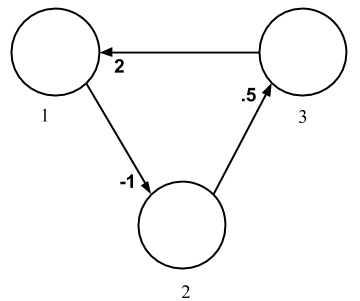
\includegraphics[scale=0.45]{./images/3NodeNet.png}
\caption[Jeff Yoshimi.]{A recurrent network with three nodes labelled $1,2,3$ and weights $w_{1,2} = -1, w_{2,3}=0.5, w_{3,1}=2$.}
\label{sampleNetRecurrent}
\end{figure}

\noindent
\stepcounter{LinearAlgebraCounter}
{\bf \theLinearAlgebraCounter.}  What is the matrix representation of the weights in the network in Fig. \ref{sampleNetRecurrent}?
{\bf Answer:}  
\[
\begin{pmatrix}
 0  &   -1 & 0 \\
 0  &   0 & 0.5 \\
 2  &   0 & 0 \\
\end{pmatrix}
\]
\bigskip

\noindent
\stepcounter{LinearAlgebraCounter}
{\bf \theLinearAlgebraCounter.}  What is the fan-in weight vector for node 2 in Fig. \ref{sampleNetRecurrent}?
{\bf Answer:}  $(-1)$. 
\bigskip

\noindent
\stepcounter{LinearAlgebraCounter}
{\bf \theLinearAlgebraCounter.}  What is
$\begin{pmatrix}1 & 1\end{pmatrix}\begin{pmatrix} 1 & 2  \\ 3 & 4 \end{pmatrix}$?
{\bf Answer:}  $\Big((1)(1) + (1)(3), (1)(2) + (1)(4)\Big)  = (4,6)$. 
\bigskip

\noindent
\stepcounter{LinearAlgebraCounter}
{\bf \theLinearAlgebraCounter.}  What is
$\begin{pmatrix}-1 & 1\end{pmatrix}\begin{pmatrix} 1 & -2  \\ 3 & 4 \end{pmatrix}$?
{\bf Answer:}  $\Big((-1)(1) + (1)(3), (-1)(-2) + (1)(4)\Big)  = (2,6)$. 
\bigskip

\noindent
\stepcounter{LinearAlgebraCounter}
{\bf \theLinearAlgebraCounter.}  What is
$\begin{pmatrix}-10 & 10\end{pmatrix}\begin{pmatrix} 0.5 & -0.5  \\ -1 &  1\end{pmatrix}$?
{\bf Answer:} $(-15,15)$. 
\bigskip


\noindent
\refstepcounter{LinearAlgebraCounter}\label{linAlgPractice1}
{\bf \theLinearAlgebraCounter.}  If the network in Fig. \ref{sampleNetRecurrent} has linear nodes and is given the activation vector $(a_1,a_2,a_3) = (1,1,1)$, what will its activation be in the next time step?
{\bf Answer:} 
\[
  \begin{matrix}\begin{pmatrix}1 & 1 & 1\end{pmatrix}\\\mbox{}\end{matrix}
 \begin{pmatrix}
 0  &   -1 & 0 \\
 0  &   0 & 0.5 \\
 2  &   0 & 0 \\
\end{pmatrix}
  =
  \bigg( (1)(0) + (1)(0) + (1)(2) ,\;\; (1)(-1) + (1)(0) + (1)(0) ,\;\; (1)(0) + (1)(.5) + (1)(0) \bigg)
  =  (2,-1,0.5)
\]
\bigskip

\noindent
\stepcounter{LinearAlgebraCounter}
{\bf \theLinearAlgebraCounter.}  If the network in Fig. \ref{sampleNetRecurrent} has linear nodes and is given the activation vector $(a_1,a_2,a_3) = (-1,-1,2)$, what will its activation be in the next time step?
{\bf Answer:} 
\[
  \begin{matrix}\begin{pmatrix}-1 & -1 & 2\end{pmatrix}\\\mbox{}\end{matrix}
 \begin{pmatrix}
 0  &   -1 & 0 \\
 0  &   0 & 0.5 \\
 2  &   0 & 0 \\
\end{pmatrix}
  =  (4,1,-0.5)
\]
\bigskip


\noindent
\refstepcounter{LinearAlgebraCounter}
{\bf \theLinearAlgebraCounter.}  If the network in question \ref{linAlgPractice1} is iterated four times, what will its activation be in those four time steps?
We saw from question \ref{linAlgPractice1} that after one time step the activation vector is $(2,-1,0.5)$. If we now use this as input to the network again we get:
\[
  \begin{matrix}
  \begin{pmatrix}2 & -1 & 0.5
  \end{pmatrix}\\\mbox{}
 \end{matrix}
 \begin{pmatrix}
 0  &   -1 & 0 \\
 0  &   0 & 0.5 \\
 2  &   0 & 0 \\
\end{pmatrix}
  =  (1,-2,-0.5)
\]
Repeating this process again with $(1,-2,-0.5)$ as input we get $(-1,-1,-1)$. Repeating one more time we get $(-2,1,-0.5)$.
{\bf Answer:}  $(2,-1,0.5),(-1,-2,-0.5),(-1,-1,-1),(-2,1,-0.5)$.
\bigskip
